\documentclass[12pt,a4paper]{report}
\usepackage{graphicx}
\graphicspath{{Pictures/}}
\usepackage{wrapfig}
\usepackage{amsmath}
\usepackage{amssymb}
\usepackage{amsthm}
\usepackage[mathscr]{euscript}
\usepackage{enumitem}
\usepackage{url}
\usepackage[T1]{fontenc}
\usepackage{color}
\definecolor{Green}{rgb}{0.00,0.40,0.00}
\usepackage{array}
\usepackage[sort,numbers]{natbib}
\usepackage{multicol}
\RequirePackage{multicol}
\usepackage[left=2.5cm,right=3cm,top=3.5cm,bottom=3cm]{geometry}
\usepackage{zref-perpage}
\zmakeperpage{footnote}
\usepackage{tocloft}
\usepackage{float}
\usepackage{caption}
\captionsetup{labelsep=colon,font=small}
\usepackage{subcaption}
\usepackage{fancyhdr}
\usepackage[colorlinks=true,citecolor=blue,urlcolor=Green]{hyperref}
\usepackage[extrafootnotefeatures]{xepersian}
\settextfont[Scale=1.3]{Yas}
\setdigitfont[Scale=1.3]{Yas}
\defpersianfont\nastaliqbig[Scale=4]{IranNastaliq}
\defpersianfont\nastaliqsmall[Scale=1]{IranNastaliq}
\swapnumbers
\theoremstyle{plain}
\newtheorem{thm}{\normalsize قضیه}[section]
\newtheorem{lem}[thm]{\normalsize لم}
\newtheorem{prop}[thm]{\normalsize گزاره}
\newtheorem{cor}[thm]{\normalsize نتیجه}
\theoremstyle{definition}
\newtheorem{defn}[thm]{\normalsize تعریف}
\newtheorem{exm}[thm]{\normalsize مثال}
\theoremstyle{remark}
\newtheorem{rem}[thm]{\normalsize تبصره}
\makeatletter\def\th@plain{\thm@notefont{}\itshape}\def\th@definition{\thm@notefont{}\normalfont}\makeatother
\renewcommand{\proofname}{\indent برهان}
\makeatletter\def\@alph#1{\ifcase#1\or صفر\or آ\or ب\or پ\or ت\or ث\or ج\or چ\or ح\or خ\or د\or ذ\or ر\or ز\or ژ\or س\or ش\or ص\or ض\or ط\or ظ\or ع\or غ\or ف\or ق\or ک\or گ\or ل\or م\or ن\or و\or هـ\or ی\else\@ctrerr\fi}\makeatother
\makeatletter\def\vhrulefill#1{\leavevmode\leaders\hrule\@height#1\hfill\kern\z@}\makeatother
\makeatletter\def\@makechapterhead#1{\vspace*{9\p@}{{\renewcommand{\baselinestretch}{1.2}\parindent\z@\flushright \normalfont\ifnum\c@secnumdepth>\m@ne\huge\bfseries\@chapapp\space\@arabic\c@chapter\par\nobreak\vskip5\p@\fi \interlinepenalty\@M\huge\bfseries#1\par\nobreak\vskip15\p@}}}\makeatother
\makeatletter\def\@makeLTRfnmark{\hbox{\@textsuperscript{\latinfont\@thefnmark}}}\renewcommand\@makefntext[1]{\parindent 1mm\noindent\hb@xt@1.8em{\hss\if@RTL\@makefnmark\else\@makeLTRfnmark\fi}#1}\makeatother
\makeatletter\def\my@makefnmark#1{\def\@tempa{#1}\ifx\@tempa\@empty\else\begingroup\unrestored@protected@xdef \@thefnmark{#1}\endgroup\fi}\let\@thefnmark\@empty
\newcommand*{\Footnote}[1]{\Footnotemark{#1}\@footnotetext}
\newcommand*{\Footnotemark}[1]{\my@makefnmark{#1}\@footnotemark}
\newcommand*{\Footnotetext}[1]{\my@makefnmark{#1}\@footnotetext}
\makeatother
\makeatletter\g@addto@macro{\UrlBreaks}{\UrlOrds}\makeatother
\renewcommand{\thesubfigure}{\alph{subfigure}}
\def\bibname{مراجع}
\def\listfigurename{\rl{فهرست شکل‌ها}}
\def\listtablename{\rl{فهرست  جدول‌ها}}
\newcommand\persianmsc[3]{#3\lr{#2}#1}
\newcommand\shamsidate[3]{#1\,/\,#2\,/\,#3}
\newcommand\talkdate[2]{#1\,--\,#2}
\def\notation#1:#2#3{#1\>\qquad\quad\quad\parbox{.8\textwidth}{#2\,\dotfill\,#3}\\[-.1pt]}
\newcommand\persiangloss[2]{#1\hfill\lr{#2}\\[-.2pt]}
\newcommand\persiansubgloss[2]{\indent#1\hfill\lr{\indent#2}\\[-.2pt]}
\newcommand\persiansubsubgloss[2]{\indent\indent#1\hfill\lr{\indent\indent#2}\\[-.2pt]}
\newcommand\englishgloss[2]{#1\hfill\rl{#2}\\}
\newcommand\englishsubgloss[2]{\indent#1\hfill\rl{\indent#2}\\}
\newcommand\termindex[2]{#1، #2\\}
\newcommand\termindexnocomma[1]{#1\\}
\newcommand\termsubindex[2]{\indent#1، #2\\}
\renewcommand\baselinestretch{1.55}
\DeclareMathOperator{\idmap}{id}
\DeclareMathOperator{\graph}{graph}
\DeclareMathOperator{\fix}{Fix}
\DeclareMathOperator{\card}{card}
%%%%%%%%%%%%%%%%%%%%%%%%%%%%%%%%%%%%%%%%%%%%%%%%%%%%%%%%% %%%%%%%%%%%%%%%%%%%%%%%%%%%%%%%%%%%%%%%%%%%%%%%%%%%%%%%%% %%%%%%%%%%%%%%%%%%%%%%%%%%%%%%%%%%%%%%%%%%%%%%%%%%%%%%%%%
\begin{document}
\vspace*{-2cm}
\pagenumbering{alph}
\thispagestyle{empty}
\begin{figure}[ht]
\centering
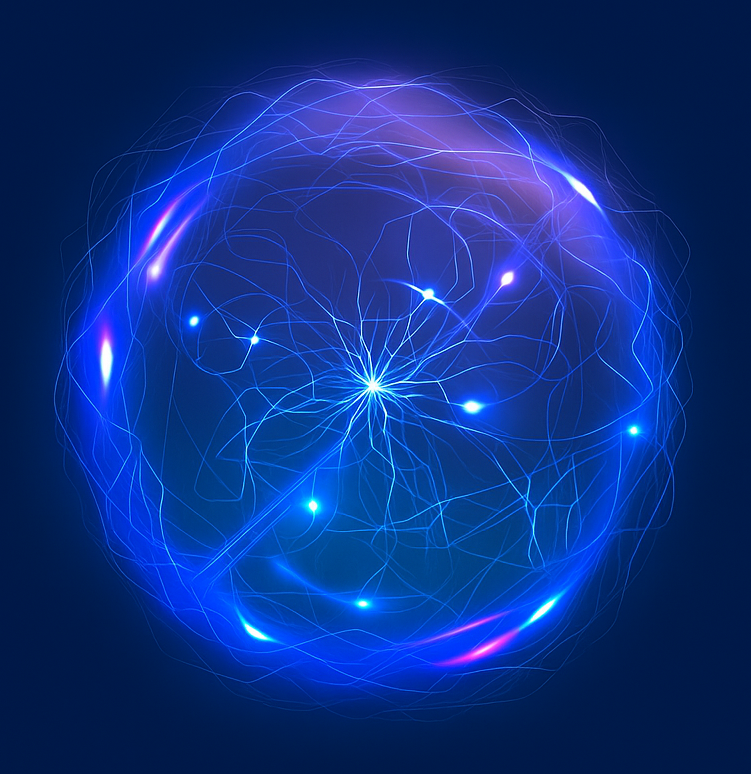
\includegraphics[width=2.5cm]{Qarm}
\end{figure}
\vspace{-0.8cm}
\begin{center}
{\nastaliqsmall مرکز تحقیقات کوانتوم شریف}\\
{\nastaliqsmall گروه الگوریتم }\vspace{1.5cm}\\
%{\LARGE پایان‌نامه‌ی کارشناسی ارشد}\\
%{\normalsize رشته - گرایش}\vspace{1.5cm}\\
{\Large عنوان:}\vspace{5mm}\\
{\Huge\textbf{ HHL}}\vspace{1.5cm}\\
{\Large پژوهشگر:}\vspace{5mm}\\
{\LARGE\textbf{جمالپور}}\vspace{1.5cm}\\
{\Large مدیرگروه :}\vspace{5mm}\\
{\LARGE\textbf{دکتر رمضانی}}\vspace{1.5cm}\\
%{\Large استاد مشاور:}\vspace{5mm}\\
%{\LARGE\textbf{دکتر ...}}\vspace{1.5cm}\\
{\Large آبان 1404}
\end{center}
%%%%%%%%%%%%%%%%%%%%%%%%%%%%%%%%%%%%%%%%%%%%%%%%%%%%%%%%% %%%%%%%%%%%%%%%%%%%%%%%%%%%%%%%%%%%%%%%%%%%%%%%%%%%%%%%%% %%%%%%%%%%%%%%%%%%%%%%%%%%%%%%%%%%%%%%%%%%%%%%%%%%%%%%%%%


%%%%%%%%%%%%%%%%%%%%%%%%%%%%%%%%%%%%%%%%%%%%%%%%%%%%%%%%% %%%%%%%%%%%%%%%%%%%%%%%%%%%%%%%%%%%%%%%%%%%%%%%%%%%%%%%%% %%%%%%%%%%%%%%%%%%%%%%%%%%%%%%%%%%%%%%%%%%%%%%%%%%%%%%%%%

%%%%%%%%%%%%%%%%%%%%%%%%%%%%%%%%%%%%%%%%%%%%%%%%%%%%%%%%% %%%%%%%%%%%%%%%%%%%%%%%%%%%%%%%%%%%%%%%%%%%%%%%%%%%%%%%%% %%%%%%%%%%%%%%%%%%%%%%%%%%%%%%%%%%%%%%%%%%%%%%%%%%%%%%%%%
\newpage
\pagestyle{fancy}
\fancyhead[RO]{\nouppercase\rightmark}
\fancyhead[LO]{\thepage}
\fancyfoot[C]{}
\renewcommand{\headrulewidth}{1pt}
\renewcommand{\footrulewidth}{0pt}
\makeatletter\renewcommand{\@starttoc}[1]{\hboxR to\textwidth{\large\textbf{عنوان}\hfill\textbf{صفحه}}\begingroup\@input{\jobname.#1}\if@filesw\expandafter\newwrite\csname tf@#1\endcsname\immediate\openout\csname tf@#1\endcsname\jobname.#1\relax\fi\@nobreakfalse\endgroup}\makeatother
\makeatletter\renewcommand*\l@chapter[2]{\ifnum\c@tocdepth>-2\relax\addpenalty{-\@highpenalty} \addvspace{4mm\@plus\p@}\setlength\@tempdima{7mm}\begingroup\parindent\z@\if@RTL\leftskip\else\rightskip\fi \@pnumwidth\parfillskip-\@pnumwidth{\leavevmode\normalsize\bfseries\textcolor{red}{فصل} #1 \hfill\hb@xt@\@pnumwidth{\hss{#2}}}\par\nobreak\global\@nobreaktrue\everypar{\global\@nobreakfalse\everypar{}} \endgroup\fi}\makeatother
\makeatletter\newcommand*\l@chapterstar[2]{\ifnum\c@tocdepth>-2\relax\addpenalty{-\@highpenalty} \addvspace{2mm\@plus\p@}\setlength\@tempdima{7mm}\begingroup\parindent\z@\if@RTL\leftskip\else\rightskip\fi \@pnumwidth\parfillskip-\@pnumwidth{\leavevmode\normalsize\bfseries\textcolor{red}{}#1 \hfill\hb@xt@ \@pnumwidth{\hss{#2}}\vspace{1.5mm}}\par\nobreak\global\@nobreaktrue\everypar{\global\@nobreakfalse\everypar{}} \endgroup\fi}\makeatother
\makeatletter\renewcommand*\l@section{\@dottedtocline{1}{4.5mm}{1.25cm}}\makeatother
\makeatletter\def\@chapter[#1]#2{\ifnum\c@secnumdepth>\m@ne\refstepcounter{chapter}\typeout{\@chapapp \space\thechapter.}\addcontentsline{toc}{chapter}{\protect\numberline{\arabic{chapter}}~~#1}\else\addcontentsline{toc}{chapter}{#1}\fi\chaptermark{#1}\addtocontents{lof}{\protect\addvspace{10\p@}}\addtocontents{lot}{\protect\addvspace{10\p@}}\if@twocolumn\@topnewpage[\@makechapterhead{#2}]\else\@makechapterhead{#2} \@afterheading\fi}\makeatother
\tableofcontents

%%%%%%%%%%%%%%%%%%%%%%%%%%%%%%%%%%%%%%%%%%%%%%%%%%%%%%%%% %%%%%%%%%%%%%%%%%%%%%%%%%%%%%%%%%%%%%%%%%%%%%%%%%%%%%%%%% %%%%%%%%%%%%%%%%%%%%%%%%%%%%%%%%%%%%%%%%%%%%%%%%%%%%%%%%%
\pagenumbering{arabic}

\chapter{}
\section*{تولید حالت کوانتومی آدیاباتیک و دانش صفر آماری}

\textbf{نویسندگان:} دوریت آهارونوف، امنون تا-شما

\subsection*{چکیده}
طراحی الگوریتم‌های کوانتومی جدید تاکنون کاری به‌غایت دشوار بوده است. این مقاله رویکردی متفاوت با مسئله در نظر می‌گیرد. ما به‌طور نظام‌مند «تولید حالت کوانتومی» را مطالعه می‌کنیم، یعنی کدام برهم نهی‌ها را می‌توان به‌صورت کارآمد تولید کرد. 

نخست نشان می‌دهیم که تمام مسائل در دانش صفر آماری \lr{(SZK)}، کلاسی که بسیاری از زبان‌های نامزد طبیعی برای BQP را در بر می‌گیرد، به یک نمونه از تولید حالت کوانتومی کاهش می‌یابند. این موضوع پیش‌تر برای ایزومورفیسم گراف شناخته شده بود، اما ما یک دستورالعمل کلی برای تمام مسائل در SZK ارائه می‌دهیم. 

کاهش از مسئله به نسخهٔ تولید حالت کوانتومی آن را برای سه مثال نشان می‌دهیم:
\begin{itemize}
	\item 
	\lr{Descrete Log}
	\item
	\lr{Quadratic residuosity}
	\item
	\lr{A gap version of closest vector in a lattice}
\end{itemize}

سپس ابزارهایی برای تولید حالت کوانتومی توسعه می‌دهیم. برای این کار، 
\begin{itemize}
	\item 
	چارچوب «تولید حالت کوانتومی آدیاباتیک» را تعریف می‌کنیم که از زبان حالت‌های پایه، گپ‌های طیفی و هامیلتونی‌ها به‌جای زبان استاندارد گیت‌های یکانی استفاده می‌کند. 
	\item
	این زبان از مدل محاسبهٔ آدیاباتیک پیشنهادشدهٔ اخیر [20] سرچشمه می‌گیرد و به‌ویژه برای کار تولید حالت کوانتومی مناسب به‌نظر می‌رسد. 
	\item
	
	پس از تعریف این الگو، دو لم بنیادی برای تولید حالت کوانتومی آدیاباتیک ارائه می‌کنیم:
	\begin{itemize}
		\item
		لم هامیلتونی تنک، که یک تکنیک کلی برای پیاده‌سازی کارآمد هامیلتونی‌های تنک می‌دهد، و
		\item
		لم مسیر آدیاباتیک ناهموار(پلکانی)، که شرایطی برای یک دنباله از هامیلتونی‌ها به‌منظور امکان تولید کارآمد حالت آدیاباتیک می‌دهد.
	\end{itemize}
\end{itemize}



از ابزارهای خود برای اثبات این موضوع استفاده می‌کنیم که هر حالت کوانتومی که بتوان در مدل استاندارد به‌صورت کارآمد تولید کرد را می‌توان به‌صورت کارآمد به‌شیوهٔ آدیاباتیک نیز تولید کرد، و برعکس. در پایان نشان می‌دهیم چگونه تکنیک‌های خود را برای تولید برهم نهی ‌های متناظر با توزیع‌های حدی دستهٔ بزرگی از زنجیره‌های مارکوف، از جمله توزیع یکنواخت روی تمام جفت‌های کامل در یک گراف دوبخشی و مجموعهٔ تمام نقاط شبکه درون اجسام محدب با بعد بالا به‌کار ببریم. این نتایج نهایی ارتباط جالبی بین محاسبات کوانتومی و زنجیره‌های مارکوف آمیخته سریع، ترسیم می‌کنند.

\section{ مقدمه}
\begin{itemize}
	\item 
	محاسبات کوانتومی می توانند مسائلی که به‌طور کلاسیک حل‌ناپذیرند را در زمان چندجمله‌ای کوانتومی حل کنند. 
	\item
	برجسته‌ترین موفقیت تاکنون الگوریتم کوانتومی شور برای فاکتورگیری اعداد صحیح و یافتن لگاریتم گسسته است [41]. 
	\item
	پس از الگوریتم شور، چند الگوریتم دیگر ارائه شدند، مانند الگوریتم هالگرن برای معادلهٔ پل [28]، الگوریتم‌های واتروس برای مدل جعبه‌سیاه گروهی [45]، و الگوریتم نماد لژاندر توسط وان دام و همکاران [14]. 
	\item
	به‌جز [14]، همهٔ این‌ها در چارچوب مسئلهٔ زیرگروه پنهان قرار می‌گیرند و در واقع دقیقاً از همان مدار کوانتومی استفاده می‌کنند؛ 
	\item
	اما [14] الگوریتمی متفاوت است اما از تبدیل‌های فوریه بهره می‌برد و ساختار جبری ویژهٔ مسئله را استفاده می‌کند. 
	\item
	اخیراً الگوریتم زیبای جدیدی توسط چایلدز و همکاران [10] یافت شد که با رویکردی کاملاً متفاوت، یعنی قدم‌زدن کوانتومی، شتاب نمایی نسبت به الگوریتم‌های کلاسیک می‌دهد؛ اما این الگوریتم در مدل جعبه‌سیاه کار می‌کند و مسئله‌ای نسبتاً ساختگی را حل می‌کند.
\end{itemize}


اهمیت توسعهٔ تکنیک‌ها و رویکردهای الگوریتمی کوانتومی از نظر کیفی متفاوت برای پیشرفت حوزهٔ محاسبات کوانتومی را نمی‌توان بیش از حد برشمرد. در این مقاله با نزدیک شدن به مسئلهٔ الگوریتم‌های کوانتومی از نقطهٔ نظر متفاوتی گامی در این جهت برمی‌داریم.
\subsection*{مسئله ایزومورفیسم گراف}
از چند سال پیش به‌طور کلی شناخته شده است که مسئلهٔ ایزومورفیسم گراف که در محاسبات کلاسیک مسئله‌ای سخت تلقی می‌شود[33]  در صورتی با یک الگوریتم کوانتومی کارآمد حل می شود که بتوان حالت کوانتومی خاصی را متناظر با آن به‌طور کارآمد تولید کرد. این حالت، برهم‌نهی همهٔ گراف‌هایی است که با یک گراف داده‌شده ایزومورف‌اند:
\begin{equation}
	|\alpha_G\rangle = \sum_{\sigma \in S_n} |\sigma(G)\rangle
\end{equation}
(برای سادگی، ثابت‌های نرمال‌ساز را در حالت بالا و در بقیهٔ مقاله نادیده می‌گیریم).
\noindent
دلیل اینکه تولید $|\alpha_G\rangle$ کافی است بسیار ساده است: برای دو گراف ایزومورف، این حالت‌ها یکسان‌اند، در حالی که برای دو گراف غیرایزومورف متعامدند. یک مدار ساده می‌تواند تمایز بین حالت متعامد و حالت یکسان را نشان دهد، که ایدهٔ اصلی آن این است که اگر حالت‌ها متعامد باشند مانع تداخل حالت‌های مختلف یک کیوبیت متصل به آن‌ها می‌شوند. وسوسه‌انگیز است فرض کنیم چنین حالتی، $|\alpha_G\rangle$، به‌آسانی ساخته می‌شود چون توزیع کلاسیک معادل، یعنی توزیع یکنواخت روی تمام گراف‌های ایزومورف با یک گراف معین، را می‌توان به‌صورت کارآمد نمونه‌برداری کرد. در واقع، حالت 
$$|\beta_G\rangle = \sum_{\sigma \in S_n} |\sigma\rangle \otimes |\sigma(G)\rangle$$
به‌آسانی با این استدلال تولید می‌شود؛ با این حال، حقیقتی کنجکاو (و آزاردهنده) از مکانیک کوانتومی این است که اگرچه $|\beta_G\rangle$ حالتی آسان برای تولید است، تاکنون کسی نمی‌داند چگونه $|\alpha_G\rangle$ را به‌صورت کارآمد تولید کند، چون نمی‌توانیم از مقدار $|\sigma\rangle$ صرف نظر کنیم.

\subsection*{Qsampling}
در این مقاله به‌طور نظام‌مند مسئلهٔ تولید حالت کوانتومی را مطالعه می‌کنیم. ما عمدتاً به نسخهٔ محدودشدهٔ تولید حالت، یعنی تولید حالت‌های متناظر با توزیع‌های احتمال کلاسیک، علاقه‌مندیم که به‌طور کلی به آن نمونه‌برداری کوانتومی (یا \lr{Qsampling}) از یک توزیع اشاره می‌کنیم. دقیق‌تر بگوییم، توزیع احتمال یک مدار $D_C$ را در نظر می‌گیریم، که توزیع روی خروجی‌های مدار کلاسیک $C$ وقتی ورودی‌هایش به‌طور یکنواخت توزیع شده‌اند است. قرار می‌دهیم 
$$|C\rangle \stackrel{\mathrm{def}}{=} \sum_{z \in \{0,1\}^m} \sqrt{D_C(z)} \,|z\rangle$$
مسئلهٔ \lr{Qsampling} مدار را تعریف می‌کنیم:
\begin{defn}[\lr{Circuit Quantum Sampling (CQS)}]:
	
ورودی: $(\epsilon, C)$ که در آن $C$ توصیفی از یک مدار کلاسیک از $n$ به $m$ بیت است، و $0 \le \epsilon \le \frac{1}{2}$.

خروجی: توصیفی از یک مدار کوانتومی $Q$ با اندازهٔ $\mathrm{poly}(|C|)$ به‌طوری که 
$$\bigl| Q(|\vec{0}\rangle) - |C\rangle \bigr| \le \epsilon$$
\end{defn}

\subsubsection*{کاهش مسائل به CQS}
نخست نشان می‌دهیم که بیشتر مسائل الگوریتمی کوانتومی تاکنون در نظر گرفته‌شده به Qsampling کاهش می‌یابند. بیشتر مسائلی که برای \lr{BQP} در نظر گرفته شده‌اند، مانند
\begin{itemize}
	\item 
	\lr{discrete log (DLOG)},
	\item
	\lr{quadratic residuosity},
	\item
	\lr{approximating closest and shortest vectors in a lattice}, 
	\item
	\lr{graph isomorphism and more},
\end{itemize}
به کلاس پیچیدگی دانش صفر آماری، یا \lr{SZK}، تعلق دارند (بخش ۲ را برای پیش‌زمینه ببینید).
ما اثبات می‌کنیم:

\begin{thm}\label{thm 1}
هر $L \in \mathrm{SZK}$ به یک خانواده از نمونه‌های \lr{CQS} کاهش می‌یابد.
\end{thm}
اثبات بر کاهش ساهای و وادهان [40] از SZK به یک مسئلهٔ کامل به نام تفاوت آماری متکی است. قضیهٔ ۱ نشان می‌دهد که یک جواب کلی برای نمونه‌برداری کوانتومی در
$\mathrm{SZK} \subseteq \mathrm{BQP}$
صدق می کند. یادآوری می‌کنیم که یک اوراکل $A$ وجود دارد که نسبت به آن $\mathrm{SZK}^A \not\subset \mathrm{BQP}^A$ [1]، و بنابراین چنین اثباتی باید 
\lr{non  relativizing}
یعنی متکی به تکنیک‌های خاص کوانتومی و ساختار داخلی مسأله باشد.

قضیهٔ ۱ یک اثبات دانش صفر را به یک نمونهٔ CQS تبدیل می‌کند. به‌طور کلی، کاهش می‌تواند نسبتاً درگیر باشد و بر کاهش در [40] استوار است. نمونه‌های خاص با علاقهٔ ویژه ساده‌تر از کار درمی‌آیند؛ مثلاً برای حالت ایزومورفیسم گراف که بالا توصیف شد، کاهش به مدار $C_G$ می‌انجامد که به‌عنوان ورودی یک رشتهٔ تصادفی یکنواخت می‌گیرد و یک گراف یکنواخت تصادفی ایزومورف با $G$ برمی‌گرداند. 

در بخش ۲، کاهش را برای سه حالت جالب نشان می‌دهیم: 

\begin{enumerate}
	\item
	یک متغیر تصمیم از DLOG (بر اساس اثبات دانش صفر گلدریچ و کوشیلویتز [21])، 
	\item
	باقی‌مانده درجه دو (بر اساس اثبات دانش صفر گلدواسر، میکالی و رکاف [24]) و 
	\item
	تقریب مسئلهٔ نزدیک‌ترین بردار در شبکه‌ها (بر اساس اثبات دانش صفر گلدریچ و گلدواسر [22]).
\end{enumerate}

موارد خاص نشان می‌دهند که اگرچه اغلب می‌توان به اثبات دانش صفر نگاه کرد و مستقیماً تولید حالت مورد نیاز را استنباط کرد، گاهی این گذار اصلاً بدیهی نیست. بااینحال قضیهٔ ۱ به ما می‌گوید چنین کاهشی همیشه ممکن است.

بنابراین، مسئلهٔ اینکه کدام حالت‌ها را می‌توان به‌صورت کارآمد توسط یک رایانهٔ کوانتومی تولید کرد  برای درک قدرت محاسباتی رایانه‌های کوانتومی اهمیت حیاتی دارد. لذا، به طراحی ابزاری برای تولید حالت کوانتومی و مطالعهٔ اینکه کدام حالت‌ها را می‌توان به‌صورت کارآمد تولید کرد می‌پردازیم. چارچوب پیشنهادشدهٔ اخیر محاسبهٔ کوانتومی آدیاباتیک [20] به‌نظر دقیقاً برای این منظور مناسب می‌رسد، چون به‌لحاظ تولید حالت کوانتومی بیان شده است؛ اجازه دهید نخست این چارچوب را توضیح دهیم.

\textbf{محاسبات کوانتومی آدیاباتیک}:
یادآوری می‌کنیم که تحول زمانی حالت یک سیستم کوانتومی $|\psi(t)\rangle$ با معادلهٔ شرودینگر توصیف می‌شود:
\begin{equation}
	i\hbar \frac{d}{dt}|\psi(t)\rangle = H(t)|\psi(t)\rangle,
\end{equation}
که در آن $H(t)$ عملگری به نام هامیلتونی سیستم است.

\noindent
سیستم‌های $n$ کیوبیتی را در نظر می‌گیریم؛ 
$H$
آنگاه محلی گرفته می‌شود، یعنی مجموعی از عملگرها که هر کدام روی تعداد ثابتی کیوبیت عمل می‌کنند. 
این محدودیت فیزیکی را در بر می‌گیرد که شامل برهم‌کنش‌های در طبیعت هستند که فقط تعداد کمی ذره را درگیر می‌کنند و به این معناست که هامیلتونی $H(t)$ در واقع در آزمایشگاه قابل پیاده‌سازی است. تحول آدیاباتیک به حالتی مربوط است که در آن $H(t)$ در زمان بسیار کند تغییر می‌کند؛ بیان کیفی قضیهٔ آدیاباتیک این است که اگر سیستم کوانتومی در حالت پایه (حالت ویژه‌ با کمترین مقدار ویژه‌) $H(0)$ مقداردهی اولیه شود، و اگر تغییر $H$ در زمان به‌اندازهٔ کافی کند، یعنی به‌صورت آدیاباتیک، انجام شود، آنگاه حالت نهایی حالت پایهٔ هامیلتونی نهایی $H(T)$ خواهد بود.

اخیراً فارحی، گلدستون، گاتمن و سیپسر [20] استفاده از تحولات آدیاباتیک را برای حل زبان‌های
\lr{NP-Hard }
پیشنهاد کردند. در [20، 15] نشان داده شد که چنین تحولات آدیاباتیکی را می‌توان به‌صورت کارآمد روی یک مدار کوانتومی شبیه‌سازی کرد، و بنابراین طراحی چنین فرایند موفقی دلالت بر یک الگوریتم کوانتومی کارآمد برای مسئله دارد. ایدهٔ فارحی و همکاران این بود که کمینهٔ یک تابع داده‌شده $f$ را به‌صورت زیر بیابند: 

$H(0)$ به‌عنوان یک هامیلتونی کلی انتخاب می‌شود. $H(T)$ به‌عنوان هامیلتونی مسئله انتخاب می‌شود، یعنی ماتریسی که مقادیر $f$ روی قطرش دارد و در بقیه صفر است. سیستم آنگاه در حالت پایهٔ $H(0)$ مقداردهی 
اولیه می‌شود و به‌صورت آدیاباتیک روی خط محدب 
$$H(t) = (1 - \frac{t}{T})H_0 + \frac{t}{T}H_T$$
تحول می‌یابد. طبق قضیهٔ آدیاباتیک اگر تحول به‌اندازهٔ کافی کند باشد، حالت نهایی حالت پایهٔ $H(T)$ خواهد بود که دقیقاً همان کمینهٔ مورد نظر $f$ است.

کارایی این الگوریتم‌های آدیاباتیک با میزان کندی لازم تحول آدیاباتیک برای برقرار بودن قضیهٔ آدیاباتیک تعیین می‌شود. معلوم می‌شود که این عمدتاً به گپ‌های طیفی هامیلتونی‌های $H(t)$ بستگی دارد. اگر این گپ‌های طیفی خیلی کوچک نباشند، تغییر هامیلتونی‌ها را می‌توان «نسبتاً سریع» انجام داد و الگوریتم آدیاباتیک آنگاه کارآمد می‌شود. مسئلهٔ اصلی در تحلیل کارایی الگوریتم‌های آدیاباتیک بنابراین کران‌گذاری پایین گپ طیفی است؛ این به‌طور کلی کاری بسیار دشوار است و از این رو از نظر تحلیلی چیز زیادی دربارهٔ الگوریتم‌های آدیاباتیک شناخته نیست. [17، 12، 18] عملکرد عددی الگوریتم‌های آدیاباتیک روی نمونه‌های تصادفی مسائل NP-کامل را تحلیل می‌کنند. در [15، 39] اثبات شد که شتاب درجه‌دو گروور [26] را می‌توان به‌صورت آدیاباتیک به‌دست آورد. کران‌های پایین برای موارد خاص در [15] داده شد. در [2] نشان داده شد که تحول آدیاباتیک با هامیلتونی‌های محلی در واقع از نظر قدرت محاسباتی معادل مدل استاندارد محاسبات کوانتومی است.

در این مقاله، استفاده از
\textbf{زبان تحولات آدیاباتیک}، 
\textbf{هامیلتونی‌ها}، 
\textbf{حالت‌های پایه}
 و 
\textbf{گپ‌های طیفی} 
را به‌عنوان چارچوب نظری برای تولید حالت کوانتومی پیشنهاد می‌کنیم. هدف ما نه جایگزینی مدل مدار کوانتومی است و نه بهبود آن، بلکه توسعهٔ یک پارادایم، یا زبان، است که در آن بتوان تولید حالت کوانتومی را به‌راحتی مطالعه کرد. مزیت استفاده از زبان هامیلتونی این است که کار تولید حالت کوانتومی طبیعی‌تر می‌شود، چون تحول آدیاباتیک به زبان تولید حالت بیان شده است. علاوه بر این، همان‌طور که خواهیم دید، به‌نظر می‌رسد این زبان بیش از مدل استاندارد مدار برای توسعهٔ ابزارهای کلی به‌کار می‌آید.

برای فراهم کردن چارچوبی برای مطالعهٔ تولید حالت با استفاده از زبان آدیاباتیک:
\begin{enumerate}
	\item 
	تولید حالت کوانتومی آدیاباتیک را تا حد امکان کلی تعریف می‌کنیم. بنابراین، شرط قرار گرفتن هامیلتونی‌ها روی یک خط راست را با هامیلتونی‌ها روی هر مسیر کلی جایگزین می‌کنیم.
	\item
	شرط محلی بودن هامیلتونی‌ها را با شرط شبیه‌سازی‌پذیر بودن آن‌ها جایگزین می‌کنیم، یعنی اینکه ماتریس یکانی $e^{-itH(s)}$ را بتوان با یک مدار کوانتومی با هر دقت چندجمله‌ای برای هر زمان $t$ کران‌دار چندجمله‌ای تقریب زد. 
\end{enumerate}
 

 بنابراین، ما هنوز از مدل استاندارد مدارهای کوانتومی در پارادایم خود استفاده می‌کنیم. با این حال، هدف ما استخراج مدارهای کوانتومی حل‌کنندهٔ مسئلهٔ تولید حالت از الگوریتم‌های تولید حالت آدیاباتیک است. در واقع، هر تولید کننده حالت آدیاباتیک را می‌توان به‌صورت کارآمد توسط یک مدار کوانتومی شبیه‌سازی کرد. دو اثبات از این موضوع می‌دهیم. اثبات اول از قضیهٔ آدیاباتیک نتیجه می‌شود. اثبات دوم خودکفا است و به دانش قضیهٔ آدیاباتیک نیاز ندارد و در عوض از اثر زنوی ساده [38] استفاده می‌کند و بنابراین دیدگاه بدیلی از الگوریتم‌های آدیاباتیک با استفاده از اندازه‌گیری‌ها ارائه می‌دهد (چنین مسیری در [11] نیز پیموده شده است). این دلالت می‌کند که مولدهای حالت آدیاباتیک را می‌توان به‌عنوان چارچوبی برای طراحی الگوریتم‌های تولید حالت کوانتومی به‌کار برد.

سپس دو ابزار بنیادی و کلی برای طراحی تولید کننده های حالت آدیاباتیک را توصیف می‌کنیم :

\textbf{پرسش اول}:
نخستین پرسشی که با آن روبرو می‌شویم به‌طور طبیعی این است که چه نوع هامیلتونی‌هایی را می‌توان به‌کار برد. به‌عبارت دیگر، چه زمانی شبیه‌سازی یا پیاده‌سازی یک هامیلتونی به‌صورت کارآمد ممکن است. برای این منظور لم هامیلتونی تنک را اثبات می‌کنیم که شرطی بسیار کلی برای شبیه‌سازی‌پذیر بودن یک هامیلتونی می‌دهد. 

\textbf{یادآوری 1}:
یک هامیلتونی $H$ روی $n$ کیوبیت سطری-تنک است اگر تعداد درایه‌های ناصفر در هر سطر آن به‌صورت چندجمله‌ای کران‌دار باشد. 

\textbf{یادآوری 2}:
$H$ 
سطری-‌محاسبه پذیر گفته می‌شود اگر الگوریتمی (کوانتومی یا کلاسیک) کارآمد وجود داشته باشد که با دادن $i$ فهرستی از $(j, H_{i,j})$ روی تمام درایه‌های ناصفر $H_{i,j}$ را برمی‌گرداند. 

\textbf{توجه}:
به‌عنوان یک نرم برای هامیلتونی‌ها از نرم طیفی استفاده می‌کنیم، یعنی نرم عملگر القاشده توسط نرم $\ell_2$ روی حالت‌ها.

\begin{lem}[لم هامیلتونی تنک]
اگر $H$ یک هامیلتونی سطری-تنک و سطری-‌محاسبه پذیر روی $n$ کیوبیت باشد و $\|H\| \le \mathrm{poly}(n)$، آنگاه $H$ قابل شبیه‌سازی‌ است.	
\end{lem}
یادآوری می‌کنیم که این لم کلی در دو زمینهٔ دیگر نیز سودمند است: نخست، در زمینهٔ شبیه‌سازی سیستم‌های فیزیکی پیچیده روی یک مدار کوانتومی؛ دوم، برای قدم‌زدن کوانتومی پیوسته [13] که از هامیلتونی‌ها استفاده می‌کند. مثلاً در [10] از هامیلتونی‌ها برای به‌دست آوردن شتاب کوانتومی نمایی با استفاده از قدم‌زدن کوانتومی استفاده شده است. لم ما را می‌توان مستقیماً برای ساده‌سازی پیاده‌سازی هامیلتونی به‌کاررفته در [10] و حذف قیود غیرضروری (یعنی رنگ‌آمیزی گره‌ها) که برای شبیه‌سازی هامیلتونی فرض شده بودند به‌کار برد.

\textbf{پرسش دوم}: 
پرسش بعدی که در طراحی الگوریتم‌های تولید حالت کوانتومی آدیاباتیک با آن روبرو می‌شود مربوط به کران‌گذاری گپ طیفی است، که همان‌طور که قبلاً گفتیم کاری دشوار است. می‌خواهیم ابزارهایی که برای یافتن مسیرهایی در فضای هامیلتونی که تضمین شده گپ‌های طیفی در آن‌ها غیرقابل چشم پوشی باشند، بکار می روند را توسعه دهیم، یعنی بزرگ‌تر از $1/\mathrm{poly}(n)$. لم بعدی ما راهی برای انجام این کار در موارد معین فراهم می‌کند. $\alpha(H)$ را حالت پایهٔ $H$ می‌نامیم (در صورت یکتا بودن).

\textbf{یادآوری 3}:
\lr{groundvalue}:
 کوچک‌ترین مقدار ویژه (انرژی حالت پایه) هر هامیلتونی $H_j$ می باشد.  به بیان دقیق‌تر، اگر مقادیر ویژه‌ی $H_j$ را با $\lambda_1 \le \lambda_2 \le \cdots$ نمایش دهیم، آنگاه:
\[
\lambda_{\min}(H_j) = \lambda_1.
\]

این یک نرمال‌سازی استاندارد است، زیرا می‌توان به هر هامیلتونی یک جمله‌ی همانی اضافه کرد:
\[
H_j \;\longrightarrow\; H_j + c I,
\]
که در آن $c$ یک ثابت است. این تبدیل بردارهای ویژه (از جمله حالت پایه) را تغییر نمی‌دهد و فقط همه‌ی مقادیر ویژه را به اندازه‌ی $c$ جابه‌جا می‌کند. بنابراین بدون کاستن از کلیت مسئله، می‌توان فرض کرد که انرژی حالت پایه صفر است.

در نتیجه، عبارت ``groundvalues 0'' یعنی همه‌ی هامیلتونی‌های دنباله طوری شیفت داده شده‌اند که انرژی حالت پایه‌ی آن‌ها صفر باشد.
\begin{lem}[لم مسیر آدیاباتیک ‌ناهموار]
	فرض کنید $\{H_j\}_{j=1}^{T=\mathrm{poly}(n)}$ دنباله‌ای از هامیلتونی‌های شبیه‌سازی‌پذیر روی $n$ کیوبیت با نرم کران‌دار چندجمله‌ای، گپ‌های طیفی غیرقابل چشم پوشی و با 
\lr{groundvalues}
	0 باشد، به‌طوری که ضرب داخلی بین حالت‌های پایهٔ یکتای $\alpha(H_j)$ و $\alpha(H_{j+1})$ برای همهٔ $j$ غیرقابل چشم پوشی باشد. آنگاه یک الگوریتم کوانتومی کارآمد وجود دارد که $\alpha(H_0)$ را تا فاصلهٔ دلخواه کوچک از $\alpha(H_T)$ می‌برد.
\end{lem}
برای اثبات این لم، ایدهٔ ساده این است که از دنبالهٔ هامیلتونی‌ها به‌عنوان سنگ‌ بنای محاسبهٔ آدیاباتیک استفاده کنیم و $H_j$ را با یک خط راست به $H_{j+1}$ وصل کنیم تا مسیر $H(t)$ را بسازیم. اما از این طریق گپ‌های طیفی در طول مسیر ممکن است کوچک شوند. در عوض از دو ایدهٔ ساده استفاده می‌کنیم که می‌توان آن‌ها را به دو ابزار سودمندتر برای دستکاری هامیلتونی‌ها برای تولید حالت آدیاباتیک تبدیل کرد. ایدهٔ اول جایگزینی هر هامیلتونی $H_j$ با هامیلتونی $\Pi_{H_j}$ است که تصویر روی زیرفضای متعامد به حالت‌های پایهٔ $H_j$ است. نحوهٔ پیاده‌سازی این تصویرگرها را با الگوریتم تخمین فاز کیتائف [32] نشان می‌دهیم. ایدهٔ دوم سودمند اتصال تصویرگرها با خطوط راست روی حالت‌هایی با ضرب داخلی غیرقابل چشم پوشی است. نشان می‌دهیم که هامیلتونی‌های روی چنین خطی گپ طیفی غیرقابل چشم پوشی دارند. این ایده‌ها را می‌توان برای نشان دادن اینکه مسیر آدیاباتیک ناهموار وصل‌کنندهٔ تصویرگرهای $\Pi_{H_j}$ گپ طیفی به‌اندازهٔ کافی بزرگ دارد ترکیب کرد.

از ابزارهای بالا برای نشان دادن این موضوع استفاده می‌کنیم که:

\begin{thm}
 هر حالت کوانتومی که بتوان در مدل مداری به‌صورت کارآمد تولید کرد را می‌توان به‌صورت کارآمد با یک الگوریتم تولید حالت آدیاباتیک نیز تولید کرد، و برعکس.

\end{thm}
بنابراین پرسش پیچیدگی تولید حالت کوانتومی (تا عبارت‌های چندجمله‌ای) در مدل مداری و در مدل تولید حالت آدیاباتیک معادل است.

در بخش پایانی مقاله نشان می‌دهیم چگونه روش‌های ما برای تولید حالت کوانتومی آدیاباتیک به‌ویژه در حوزهٔ جالب، یعنی Qsampling از توزیع‌های حدی زنجیره‌های مارکوف، کار می‌کنند. ارتباط جالبی بین زنجیره‌های مارکوف آمیخته سریع و محاسبهٔ آدیاباتیک وجود دارد. یک زنجیرهٔ مارکوف آمیخته سریع است اگر و تنها اگر گپ مقدار ویژه‌ دوم، یعنی تفاوت بین بزرگ‌ترین و دومین بزرگ‌ترین مقدار ویژه‌ ماتریس مارکوف $M$، غیرقابل چشم پوشی باشد [4]. این آشکارا شباهت به شرط آدیاباتیک گپ طیفی غیرقابل چشم پوشی دارد و پیشنهاد می‌کند به هامیلتونی‌های به‌صورت 
\begin{equation}\label{eq3}
	H_M = I - M
\end{equation}
نگاه کنیم. $H_M$ یک هامیلتونی خواهد بود اگر $M$ متقارن باشد؛ اگر $M$ متقارن نباشد اما یک زنجیرهٔ مارکوف برگشت‌پذیر [35] باشد هنوز می‌توانیم هامیلتونی متناظر با آن را تعریف کنیم (بخش ۸ را ببینید). لم هامیلتونی تنک وقتی سریعا نتیجهٔ می دهد که برای نوع ویژه‌ای از زنجیره‌های مارکوف، که آن‌ها را نمونه‌برداری‌پذیر قوی می‌نامیم، آنالوگ کوانتومی زنجیرهٔ مارکوف قابل پیاده‌سازی است:

\begin{cor}
اگر $M$ یک زنجیرهٔ مارکوف نمونه‌برداری‌پذیر قوی باشد، آنگاه $H_M$ شبیه‌سازی‌پذیر است.
\end{cor}
در محاسبات آدیاباتیک به دنباله‌های هامیلتونی‌ها علاقه‌مندیم؛ بنابراین دنباله‌های زنجیره‌های مارکوف نمونه‌برداری‌پذیر قوی را در نظر می‌گیریم. در مطالعهٔ زنجیره‌های مارکوف پارادایم به‌ویژه جالبی وجود دارد که در آن از دنباله‌های زنجیره‌های مارکوف تکراری استفاده می‌شود: شمارش تقریبی [30]. در شمارش تقریبی ایده این است که از یک زنجیرهٔ مارکوف روی مجموعه‌ای که به‌آسانی قابل شمارش است و در یک مجموعهٔ بزرگ $\Omega$ که اندازهٔ آن را می‌خواهیم تخمین بزنیم قرار دارد شروع کنیم؛ سپس به‌آهستگی مجموعهٔ روی آن زنجیرهٔ مارکوف عمل می‌کند را افزایش می‌دهیم تا در نهایت به مجموعهٔ مورد نظر $\Omega$ برسیم. این پارادایم و تغییرات آن، که در آن زنجیره‌های مارکوف اندکی تغییر می‌کنند تا زنجیرهٔ مارکوف مورد نظر حاصل شود، ابزار متداولی در بسیاری از الگوریتم‌هاست؛ نمونهٔ برجسته الگوریتم اخیر برای تقریب permanent [29] است. در بخش آخر مقاله نشان می‌دهیم چگونه از تکنیک‌های خود برای تبدیل چنین الگوریتم‌های شمارش تقریبی به‌منظور نمونه‌برداری کوانتومی از توزیع‌های حدی زنجیرهٔ مارکوف نهایی استفاده کنیم. نشان می‌دهیم:
\begin{thm}[به‌ تعبیری :]
فرض کنید $A$ یک الگوریتم تصادفی کارآمد برای شمارش تقریبی یک مجموعهٔ $\Omega$ احتمالاً وزندار باشد؛ فرض کنید $A$ از زنجیره‌های مارکوف به‌آهستگی تغییرکننده که از یک زنجیرهٔ مارکوف ساده شروع می‌شوند استفاده می‌کند. آنگاه یک الگوریتم کوانتومی کارآمد $Q$ وجود دارد که از توزیع حدی نهایی روی $\Omega$ Qsample می‌گیرد.
\end{thm}
تأکید می‌کنیم که اینطور نیست که به شتاب کوانتومی برای نمونه‌برداری از توزیع‌های گوناگون علاقه‌مند باشیم بلکه به Qsample همدوس توزیع کلاسیک علاقه‌مندیم.

از این پارادایم برای Qsample از مجموعهٔ تمام جفت‌های کامل یک گراف دوبخشی با استفاده از الگوریتم اخیر جروم، سینکلر و ویگودا [29] بهره می‌بریم. با همان ایده‌ها می‌توانیم از تمام توسیع‌های خطی ترتیب‌های جزئی با الگوریتم بوبلی و دایر [9]، از تمام نقاط شبکه در یک جسم محدب با شرایط معین با تکنیک اپلگیت-کانان [6] و از حالت‌های بسیار دیگر Qsample بگیریم. یادآوری می‌کنیم که برخی از این حالت‌ها (شاید همه) را می‌توان با تکنیک‌های استاندارد که خودکاهش‌پذیری مسئله را استثمار می‌کنند تولید کرد (ببینید [27]). با این حال تأکید می‌کنیم که تکنیک‌های ما از نظر کیفی و به‌طور قابل توجهی با تکنیک‌های قبلی برای تولید حالت‌های کوانتومی متفاوت‌اند و به‌ویژه به خودکاهش‌پذیری نیاز ندارند. این می‌تواند برای گسترش این رویکرد به حالت‌های کوانتومی دیگر مهم باشد.

در این مقاله پایه‌های مطالعهٔ کلی مسئلهٔ Qsampling و تولید حالت کوانتومی آدیاباتیک را بنا نهادیم، که در آن استفاده از زبان هامیلتونی‌ها و حالت‌های پایه را برای تولید حالت کوانتومی پیشنهاد کردیم. این جهت به ارتباطات بسیار جالب و جذاب بین محاسبات کوانتومی و حوزه‌های گوناگون اشاره دارد: کلاس پیچیدگی SZK و مسئلهٔ کامل آن تفاوت آماری [40]， مفهوم تحول آدیاباتیک [31]， مطالعهٔ زنجیره‌های مارکوف با اختلاط سریع با استفاده از گپ‌های طیفی [35]， قدم‌زدن کوانتومی [10]، و مطالعهٔ حالت‌های پایه و گپ‌های طیفی هامیلتونی‌ها در فیزیک. امیدواریم این ارتباطات به تکنیک‌های گوناگون از این حوزه‌ها اشاره کنند که بتوان برای تولید ابزارهای بیشتر برای تولید حالت آدیاباتیک وام گرفت؛ به‌ویژه، مطالعهٔ گپ‌های طیفی هامیلتونی‌ها در فیزیک حوزهٔ پرجنب‌وجوشی با تکنیک‌های توسعه‌یافتهٔ اخیر است (ببینید [42] و مراجع آن). به‌نظر می‌رسد درک بسیار عمیق‌تری از پارادایم آدیاباتیک برای حل جالب‌ترین پرسش باز، یعنی طراحی الگوریتم‌های کوانتومی جدید جالب، لازم است. پرسش بازی که ممکن است در این کار کمک کند ارائهٔ الگوریتم‌های کوانتومی شناخته‌شده، مثلاً الگوریتم DLOG شور یا الگوریتم باقی‌ماندگی درجه دو، به زبان محاسبهٔ آدیاباتیک به‌شیوهٔ بینش‌آور است.

بقیهٔ مقاله به‌صورت زیر سازماندهی شده است. با نتایج مربوط به SZK شروع می‌کنیم؛ سپس محاسبهٔ کوانتومی آدیاباتیک را توصیف می‌کنیم، چارچوب تولید حالت کوانتومی آدیاباتیک را تعریف می‌کنیم و از قضیهٔ آدیاباتیک برای اثبات اینکه یک مولد حالت آدیاباتیک دلالت بر یک الگوریتم تولید حالت دارد استفاده می‌کنیم. سپس دو ابزار اصلی خود را اثبات می‌کنیم: لم هامیلتونی تنک و لم مسیر آدیاباتیک ناهموار. سپس از این ابزارها برای اثبات معادل بودن تولید حالت آدیاباتیک و تولید حالت کوانتومی استاندارد استفاده می‌کنیم. در پایان ارتباط با زنجیره‌های مارکوف را ترسیم می‌کنیم و نشان می‌دهیم چگونه از تکنیک‌های خود برای Qsample از مجموعه‌های قابل شمارش تقریبی استفاده کنیم. در پیوست اثبات دوم تبدیل مولدهای حالت آدیاباتیک به الگوریتم‌ها با استفاده از اثر زنو را می‌دهیم.

\section{ Qsampling و SZK}

با مقداری پیش‌زمینه دربارهٔ دانش صفر آماری شروع می‌کنیم. برای منبعی عالی دربارهٔ این موضوع، تز وادهان [44] یا ساهای و وادهان [40] را ببینید.

\subsection{SZK}

یک زوج $\Pi = (\Pi_{\mathrm{Yes}}, \Pi_{\mathrm{No}})$ یک 
\lr{promise problem}
 است اگر $\Pi_{\mathrm{Yes}} \subseteq \{0,1\}^*$، $\Pi_{\mathrm{No}} \subseteq \{0,1\}^*$ و $\Pi_{\mathrm{Yes}} \cap \Pi_{\mathrm{No}} = \emptyset$. $\Pi_{\mathrm{Yes}}$ را به‌عنوان مجموعهٔ تمام نمونه‌های بله و $\Pi_{\mathrm{No}}$ را به‌عنوان مجموعهٔ تمام نمونه‌های خیر در نظر می‌گیریم و به بقیهٔ ورودی‌ها کاری نداریم. اگر هر $x \in \{0,1\}^*$ در $\Pi_{\mathrm{Yes}} \cup \Pi_{\mathrm{No}}$ باشد آن را یک زبان می‌نامیم.

می‌گوییم یک مسئلهٔ \lr{promise} $\Pi$ یک اثبات تعاملی با خطای صدق $\epsilon_s$ و خطای کامل بودن $\epsilon_c$ دارد اگر پروتکل تعاملی بین اثبات‌کنندهٔ $P$ و بررسی‌کنندهٔ $V$ با نماد $(P,V)$ وجود داشته باشد، که در آن $V$ یک ماشین احتمالی با زمان چندجمله‌ای است، و 
\begin{enumerate}
	\item 
	اگر $x \in \Pi_{\mathrm{Yes}}$ آنگاه $V$ با احتمال حداقل $1 - \epsilon_c$ می‌پذیرد؛ 
	\item
	اگر $x \in \Pi_{\mathrm{No}}$ آنگاه برای هر اثبات‌کنندهٔ $P^*$، $V$ با احتمال حداکثر $\epsilon_s$ می‌پذیرد. 
\end{enumerate}
وقتی یک سیستم اثبات تعاملی $(\Pi, V)$ برای یک مسئلهٔ \lr{promise} $\Pi$ روی ورودی $x$ اجرا می‌شود، توزیعی روی «رونوشت‌ها» تولید می‌کند که مکالمهٔ بین اثبات‌کننده و بررسی‌کننده را در بر می‌گیرند؛ یعنی هر رونوشت ممکن با احتمالی (وابسته به پرتاب سکهٔ تصادفی اثبات‌کننده و بررسی‌کننده) ظاهر می‌شود.

\textbf{توضیح}: 
	در این متن، صحبت از \textbf{اثبات‌های تعاملی} است که در 
\lr{promise problems}
	 مورد استفاده قرار می‌گیرند. بیایید این موضوع را به طور گام به گام توضیح دهیم:
	
	\begin{enumerate}
		\item \textbf{مسئلهٔ \lr{promise}} 
		(\(\Pi\)):
		 همان‌طور که قبلاً توضیح دادیم، مسئلهٔ \lr{promise} (\(\Pi = (\Pi_{\text{Yes}}, \Pi_{\text{No}})\)) یک مسئله است که در آن ورودی‌ها به دو مجموعه تقسیم می‌شوند: ورودی‌های «بله» و ورودی‌های «نه». در اینجا، هدف از اثبات تعاملی این است که نشان دهیم برای ورودی‌های بله، بررسی‌کننده باید با احتمال بالا جواب «بله» بدهد، و برای ورودی‌های نه، احتمال خطا در پذیرش باید کم باشد.
		
		\item \textbf{اثبات تعاملی}: در اینجا، اثبات‌کننده (که به آن \(P\) گفته می‌شود) و بررسی‌کننده (که به آن \(V\) گفته می‌شود) با هم تعامل می‌کنند. بررسی‌کننده یک ماشین احتمالی با زمان چندجمله‌ای است. به عبارت ساده‌تر، بررسی‌کننده یک برنامه است که با استفاده از احتمال (شبیه به یک پرتاب سکه) تصمیم می‌گیرد که آیا ورودی را قبول کند یا نه.
		
		\item \textbf{خطای صدق و خطای کامل بودن}:
		\begin{itemize}
			\item \textbf{خطای صدق} (\(\epsilon_s\)): وقتی ورودی در مجموعه \(\Pi_{\text{No}}\) قرار دارد، بررسی‌کننده باید تقریباً همیشه (با احتمال کمتر از \(\epsilon_s\)) رد کند. این خطا به این معنی است که بررسی‌کننده نباید ورودی‌های نادرست را به اشتباه قبول کند.
			\item \textbf{خطای کامل بودن} (\(\epsilon_c\)): وقتی ورودی در مجموعه \(\Pi_{\text{Yes}}\) قرار دارد، بررسی‌کننده باید تقریباً همیشه (با احتمال بیشتر از \(1 - \epsilon_c\)) قبول کند. این خطا به این معنی است که برای ورودی‌های درست (که در مجموعه بله قرار دارند)، بررسی‌کننده باید این ورودی‌ها را با احتمال بالا قبول کند.
		\end{itemize}
		
		\item \textbf{پروتکل تعاملی}: در پروتکل تعاملی، اثبات‌کننده و بررسی‌کننده به نوبت پیام‌هایی را برای هم ارسال می‌کنند. این پروتکل شامل چندین دور مکالمه است که در هر دور، اثبات‌کننده و بررسی‌کننده تصمیم می‌گیرند چه پیامی رد و بدل کنند. در هر مکالمه، بررسی‌کننده ممکن است از احتمال (مثلاً پرتاب سکه) برای تصمیم‌گیری استفاده کند.
		
		\item \textbf{رونوشت‌ها}: رونوشت‌ها به مجموعه‌ای از پیام‌ها یا مکالمات بین اثبات‌کننده و بررسی‌کننده اطلاق می‌شود. در واقع، هر رونوشت ممکن است با احتمال خاصی (که به عملکرد تصادفی اثبات‌کننده و بررسی‌کننده بستگی دارد) تولید شود. این توزیع‌های رونوشت‌ها نشان می‌دهند که چگونه مکالمه‌ها بین اثبات‌کننده و بررسی‌کننده در پروتکل تعاملی به وقوع می‌پیوندند.
	\end{enumerate}
	
	در مجموع، این متن به نحوه کار یک اثبات تعاملی برای مسئلهٔ وعده‌ای اشاره دارد که در آن بررسی‌کننده تصمیم می‌گیرد که آیا ورودی متعلق به مجموعه "بله" است یا نه. این تصمیم‌گیری با استفاده از یک پروتکل تعاملی و احتمال‌های خاص برای پذیرش ورودی‌ها انجام می‌شود.
	
یک سیستم اثبات تعاملی $(\Pi, V)$ برای یک
 \lr{promise problem}، $\Pi$ 
«دانش صفر آماری بررسی‌کنندهٔ صادق» گفته می‌شود، و به‌اختصار HVSZK، اگر یک شبیه‌ساز احتمالی با زمان چندجمله‌ای $S$ وجود داشته باشد که برای هر $x \in \Pi_{\mathrm{Yes}}$ توزیعی روی رونوشت‌ها تولید کند که به توزیع رونوشت‌ها در اثبات واقعی نزدیک (در فاصلهٔ $\ell_1$ تعریف‌شدهٔ زیر) باشد. اگر توزیع شبیه‌سازی‌شده دقیقاً توزیع صحیح باشد، می‌گوییم سیستم اثبات «دانش صفر کامل بررسی‌کنندهٔ صادق» است، و به‌اختصار \lr{HVPZK}.

تأکید می‌کنیم که خروجی شبیه‌ساز فقط بر اساس ورودی است و شبیه‌ساز به اثبات‌کننده دسترسی ندارد. همچنین توجه کنید که فقط لازم است شبیه‌ساز برای ورودی‌های در $\Pi_{\mathrm{Yes}}$ توزیع خوبی تولید کند و به ورودی‌های دیگر کاری نداریم، چون برای نمونه‌های «خیر» به‌هرحال اثبات صحیحی وجود ندارد. خوانندهٔ علاقه‌مند را به تز وادهان [44] برای تعاریف دقیق و بحث دربارهٔ ظرافت‌های آن‌ها ارجاع می‌دهیم.

تعریف \lr{HVSZK} دقیقاً مفهوم «دانش صفر» را در بر می‌گیرد: اگر بررسی‌کنندهٔ صادق بتواند تعامل با اثبات‌کننده را در صورت بودن ورودی در $\Pi$ خودش شبیه‌سازی کند، آنگاه از تعامل چیزی یاد نمی‌گیرد (جز این دانش که ورودی در $\Pi$ است). با \lr{HVSZK} کلاس تمام 
\lr{promise problems}
 را که اثبات تعاملی با این محدودیت‌ها دارند نشان می‌دهیم. می‌توان پرسید آیا بررسی‌کننده‌های متقلب می‌توانند با انحراف از پروتکل از اثبات‌کنندهٔ صادق اطلاعات بگیرند. در واقع در برخی اثبات‌های تعاملی این اتفاق می‌افتد. با این حال یک نتیجهٔ کلی می‌گوید هر اثبات HVSZK را می‌توان با اثباتی شبیه‌سازی کرد که حتی با بررسی‌کننده‌های غیرصادق اطلاعات زیادی افشا نمی‌کند [23]. بنابراین با SZK کلاس تمام \lr{promise problems} را که سیستم‌های اثبات تعاملی دانش صفر آماری نسبت به بررسی‌کنندهٔ صادق (یا معادلاً کلی) دارند نشان می‌دهیم.

معلوم است که $\mathrm{BPP} \subseteq \mathrm{SZK} \subseteq \mathrm{AM} \cap \mathrm{coAM}$ و SZK تحت متمم بسته است. در نتیجه SZK هیچ زبان NP-کاملی را در بر نمی‌گیرد مگر آنکه سلسله‌مراتب چندجمله‌ای فرو بریزد. برای این و سایر نتایج شناخته‌شده دربارهٔ این کلاس ظریف، دوباره خواننده را به تز وادهان [44] ارجاع می‌دهیم.
\subsection{ مسئلهٔ کامل}

اخیراً ساهای و وادهان مسئلهٔ طبیعی کاملی برای کلاس دانش صفر آماری، با نماد \lr{SZK}، یافتند. نکتهٔ خوب دربارهٔ این مسئله این است که به هیچ وجه به‌صورت صریح یا ضمنی به اثبات‌های تعاملی اشاره نمی‌کند. برای تعریف مسئله به چند واقعیت دربارهٔ فاصلهٔ بین توزیع‌ها نیاز داریم. برای دو توزیع کلاسیک $\{p(x)\}$، $\{q(x)\}$ فاصلهٔ $\ell_1$ و وفاداری آن‌ها را تعریف می‌کنیم (این معیار با نام‌های دیگر نیز شناخته می‌شود):
\[
|p - q|_1 = \sum_x |p(x) - q(x)|, \qquad
F(p,q) = \sum_x \sqrt{p(x) q(x)}.
\]
همچنین فاصلهٔ تغییر را $||p - q|| = \frac{1}{2}|p - q|_1$ تعریف می‌کنیم تا مقداری بین ۰ و ۱ باشد. واقعیت زیر بسیار سودمند است:

\textbf{واقعیت ۱.} (ببینید [37])
\[
1 - F(p,q) \le ||p - q|| \le \sqrt{1 - F(p,q)^2}
\]
یا معادل آن
\[
1 - ||p - q|| \le F(p,q) \le \sqrt{1 - ||p - q||^2}.
\]

اکنون می‌توانیم مسئلهٔ کامل برای SZK را تعریف کنیم:
\begin{defn}[تفاوت آماری $SD_{\alpha,\beta}$]
\noindent
\begin{itemize}
	\item 
	\textbf{ورودی}: دو مدار کلاسیک $C_0$, $C_1$ با $m$ خروجی بولی.
	\item
	\textbf{promize}: $||D_{C_0} - D_{C_1}|| \ge \alpha$ یا $||D_{C_0} - D_{C_1}|| \le \beta$.
	\item
	\textbf{خروجی}: کدام یک از دو امکان رخ می‌دهد؟ (بله برای مورد اول و خیر برای مورد دوم)
\end{itemize}
\end{defn}
ساهای و وادهان [40، 44] نشان می‌دهند که برای هر دو ثابت $0 \le \beta < \alpha \le 1$ به‌طوری که حتی $\alpha^2 > \beta$، $SD_{\alpha,\beta}$ برای SZK کامل است. توضیحی خوش‌بیان را نیز می‌توان در [44] یافت.

\subsection{ تقلیل از SZK به Qsampling}
به یک بلوک سازندهٔ بسیار ساده نیاز داریم.

\textbf{ادعا ۱.} فرض کنید $\psi = \frac{1}{\sqrt{2}}(|0,v\rangle + |1,w\rangle)$. اگر یک گیت هادامارد روی کیوبیت اول اعمال کنیم و آن را اندازه بگیریم، با احتمال $\frac{1 + \mathrm{Real}(\langle v|w\rangle)}{2}$ پاسخ ۰ و با احتمال $\frac{1 - \mathrm{Real}(\langle v|w\rangle)}{2}$ پاسخ ۱ را می‌گیریم.

اثبات یک محاسبهٔ مستقیم است. اکنون به اثبات قضیهٔ \ref{thm 1} می‌پردازیم.
\begin{proof}
 فرض کنید $C_0$, $C_1$ ورودی \lr{SD} باشند؛ $C_0$, $C_1$ مدارهایی با $m$ خروجی‌اند. کافی است نشان دهیم که با فرض توانایی \lr{Qsample} از مدارهای داده‌شده،
$SD_{1/4,3/4} \in \mathrm{BQP}$.

نخست فرض کنیم می‌توانیم از هر دو مدار با خطای $\epsilon = 0$ Qsample بگیریم. بنابراین می‌توانیم برهم نهی $\frac{1}{\sqrt{2}}(|0\rangle |C_0\rangle + |1\rangle |C_1\rangle)$ را تولید کنیم. سپس یک گیت هادامارد روی کیوبیت اول اعمال می‌کنیم و آن را اندازه می‌گیریم. از ادعا ۱ با $v = |C_0\rangle$ و $w = |C_1\rangle$ استفاده می‌کنیم. در حالت ما

\begin{equation}
	\langle v|w\rangle = \sum_{z \in \{0,1\}^m} \sqrt{D_{C_0}(z) D_{C_1}(z)} = F(D_{C_0}, D_{C_1})
\end{equation}

بنابراین با احتمال $\frac{1 + F(D_{C_0}, D_{C_1})}{2}$ مقدار ۰ می‌گیریم. پس
\begin{itemize}
	\item 
	 اگر $||D_{C_0} - D_{C_1}|| \ge \alpha$ آنگاه با احتمال $\frac{1 + \sqrt{1 - ||D_{C_0} - D_{C_1}||^2}}{2} \le \frac{1 + \sqrt{1 - \alpha^2}}{2}$ مقدار ۰ اندازه می‌گیریم؛ در حالی که 
	\item
	اگر $||D_{C_0} - D_{C_1}|| \le \beta$ آنگاه با احتمال $\frac{2 - ||D_{C_0} - D_{C_1}||}{2} \ge 1 - \frac{\beta}{2}$ مقدار ۰ اندازه می‌گیریم.
\end{itemize}

 با قرار دادن $\alpha = \frac{3}{4}$ و $\beta = \frac{1}{4}$ اگر $||D_{C_0} - D_{C_1}|| \ge \alpha$ با احتمال حداکثر 
$$\frac{1 + \sqrt{1 - \alpha^2}}{2} \le 0.831$$
 مقدار ۰ اندازه می‌گیریم، در حالی که اگر $||D_{C_0} - D_{C_1}|| \le \beta$ با احتمال حداقل 
 $$1 - \frac{\beta}{2} \ge \frac{7}{8} = 0.875$$
 مقدار ۰ اندازه می‌گیریم. با تکرار آزمایش $O(\log(1/\delta))$ بار می‌توانیم با احتمال خطای کمتر از $\delta$ به پاسخ درست برسیم. اگر مدار نمونه‌برداری کوانتومی خطای کوچکی داشته باشد (مثلاً $\epsilon < \frac{1}{100}$) آنگاه حالت‌های حاصل به حالت‌های صحیح نزدیک‌اند و خطای ایجادشده را می‌توان در گپ الگوریتم BQP بلعید.
\end{proof}
قضیهٔ بالا نشان می‌دهد که برای دادن یک الگوریتم کوانتومی کارآمد برای هر مسئله در SZK کافی است یک نمونه‌بردار کوانتومی کارآمد از مدارهای متناظر پیدا کنیم. می‌توان از قضیه برای شروع از یک اثبات دانش صفر برای یک زبان معین و تبدیل آن به خانوادهٔ مدارهایی که می‌خواهیم از آن‌ها Qsample بگیریم استفاده کرد. گاهی این کاهش می‌تواند بسیار آسان باشد، بدون نیاز به گذر از تقلیل پیچیدهٔ ساهای و وادهان [40]، اما به‌طور کلی نمی‌دانیم که مشخصهٔ حالت‌ها به‌آسانی استخراج شود. برای توضیح، توصیف‌های دقیق حالت‌های مورد نیاز برای Qsample را برای سه مثال می‌دهیم که در آن‌ها کاهش بسیار ساده‌تر از حالت کلی از کار درمی‌آید. این موارد به‌ویژه برای الگوریتم‌های کوانتومی مورد علاقه‌اند: لگاریتم گسسته، باقی‌ماندگی درجه دو و نسخهٔ گپی از نزدیک‌ترین بردار در یک شبکه.

\subsection{یک  \lr{promise problem} معادل با لگاریتم گسسته}
\textbf{مسئله}: گلدریچ و کوشیلویتز [21] مسئلهٔ وعدهٔ
$DLP_c$ 
را به‌صورت زیر تعریف می‌کنند:
\begin{itemize}
	\item 
	\textbf{ورودی}: یک عدد اول $p$، یک مولد $g$ از $\mathbb{Z}_p^*$ و ورودی $y \in \mathbb{Z}_p^*$.
	\item
	\textbf{promise}:
	 \textbf{promise} این است که $x = \log_g(y)$ در $[1, cp] \cup [\frac{p}{2}+1, \frac{p}{2}+cp]$ است.
	\item
	\textbf{خروجی}: آیا $x \in [1, cp]$ است یا $x \in [\frac{p}{2}+1, \frac{p}{2}+cp]$؟
\end{itemize}
[21] اثبات می‌کند که \lr{DLOG} برای هر $0 < c < 1/2$ به
$DLP_c$ 
کاهش می‌یابد. آن‌ها همچنین اثبات می‌کنند که
$DLP_c$ 
اگر $0 < c \le 1/6$ باشد اثبات دانش صفر کامل دارد. ما $c = 1/6$ می‌گیریم و نشان می‌دهیم چگونه
$DLP_{1/6}$
  را با \lr{CQS} حل کنیم.

\textbf{کاهش}:
 فرض می‌کنیم می‌توانیم مسئلهٔ ساخت را برای مدار $C_{y,k} = C_{n,g,y,k}$ که
  $$C_{y,k}(i) = y \cdot g^i \pmod{p}$$
  را برای $i \in \{0,1\}^k$ 
 محاسبه می‌کند حل کنیم. الگوریتم به حالت 
 $$\frac{1}{\sqrt{2}}\bigl[ |0\rangle |C_{g^{p/2+1},\lfloor \log p \rfloor - 1}\rangle + |1\rangle |C_{y,\lfloor \log p \rfloor - 3}\rangle \bigr]$$ 
 می‌رود و طبق ادعای ۱ ادامه می‌دهد.

\textbf{درستی}:
 داریم
  \begin{equation}\label{eq5}
  	|C_{g^{p/2+1},\lfloor \log p \rfloor - 1}\rangle = \frac{1}{\sqrt{2^t}} \sum_{i=0}^{2^t - 1} |g^{p/2 + i}\rangle
  \end{equation}
 که $t$ بزرگترین توان ۲ کوچکتر از $p$ است. همچنین چون $y = g^x$ داریم 
\begin{equation}\label{eq6}
	 |C_{y,\lfloor \log p \rfloor - 3}\rangle = \frac{1}{\sqrt{2^{t'}}} \sum_{i=0}^{2^{t'}-1} |g^{x+i}\rangle
\end{equation}
 که $t'$ بزرگترین توان ۲ کوچکتر از $p/8$ است. اکنون با مقایسهٔ توان‌های $g$ در پشتیبانی معادلات \eqref{eq5} و \eqref{eq6} می‌بینیم که 
 \begin{itemize}
 	\item 
 	اگر $x \in [1, cp]$ آنگاه
 	\[\left| {{C_{{g^{p/2 + 1}},\left\lfloor {\log p} \right\rfloor  - 1}}} \right\rangle ,\,\,\,\,and\,\,\,\,\left| {{C_{y,\left\lfloor {\log p} \right\rfloor  - 3}}} \right\rangle \]
 	پشتیبانی‌های مجزا دارند و بنابراین
 	$$\langle C_{y,\lfloor \log p \rfloor - 3} | C_{g^{p/2+1},\lfloor \log p \rfloor - 1} \rangle = 0$$
 	\item
 	 در حالی که اگر $x \in [\frac{p}{2}+1, \frac{p}{2}+cp]$ آنگاه همپوشانی بزرگ است و
 	$$|\langle C_{y,\lfloor \log p \rfloor - 3} | C_{g^{p/2+1},\lfloor \log p \rfloor - 1} \rangle|$$ 
 	ثابت است.
 \end{itemize}
\subsection{باقی‌مانده درجه دو}
\textbf{مسئله} : 
اگر $x = y^2 \pmod{n}$ برای برخی مقادیر $y$ باشد $x R n$ می‌نویسیم و در غیر این صورت $x N n$. مسئلهٔ QR این است که روی ورودی
$x$
 و
$n$ 
تصمیم بگیریم آیا $x R n$ هست یا خیر ؟ برای حالتیکه $n$ اول باشد الگوریتم کارآمدی شناخته شده است و مسئله برای $n = pq$ که
$p$
و
$q$ 
به‌طور تصادفی از بین اعداد اول بزرگ انتخاب شده‌اند سخت فرض می‌شود. واقعیت بنیادی که مستقیماً از قضیهٔ باقی‌ماندهٔ چینی نتیجه می‌شود:

\textbf{واقعیت ۲.}
\begin{itemize}
	\item 
	اگر فاکتورگیری اول از $n$ برابر $n = p_1^{e_1} p_2^{e_2} \cdots p_k^{e_k}$ باشد، آنگاه برای هر $x$ داریم 
	$$x R n \Leftrightarrow \forall_{1 \le i \le k} \; x R p_i$$
	\item
	اگر فاکتورگیری اول از $n$ برابر $n = p_1 p_2 \cdots p_k$ باشد آنگاه هر $z \in \mathbb{Z}_n$ که ریشهٔ مربع دارد، همان تعداد ریشهٔ مربع را دارد.
\end{itemize}
نشان می‌دهیم چگونه حالت $n = pq$ را به CQS کاهش دهیم (با اتخاذ اثبات دانش صفر [24]).

\textbf{کاهش}:
 از مدار $C_a(r)$ استفاده می‌کنیم که روی ورودی 
$r \in \mathbb{Z}_n$
  خروجی
$$z = r^2 a \pmod{n}$$
 را می‌دهد. فرض کنید برای هر $a$ بدانیم چگونه از $C_a$ نمونه‌برداری کوانتومی کنیم. روی ورودی اعداد صحیح 
 $n$،
  $x$ 
  و
 $(n,x) = 1$،
  الگوریتم به حالت $\frac{1}{\sqrt{2}}[|0\rangle |C_1\rangle + |1\rangle |C_x\rangle]$ می‌رود و طبق ادعای ۱ ادامه می‌دهد.

\textbf{درستی}:
 داریم
  \begin{equation}\label{eq7}
  	|C_x\rangle = \sum_z \sqrt{p_z} |z\rangle
  \end{equation} 
 که $p_z = \Pr_r(z = r^2 x)$ و
  \begin{equation}\label{eq8}
  	|C_1\rangle = \sum_{z: z R n} \alpha |z\rangle
  \end{equation}
 برای مقداری $\alpha$ ثابت مستقل از $z$. 
 \begin{itemize}
 	\item 
 	 اگر $x R n$ آنگاه $z = r^2 x$ نیز یک مربع است. علاوه بر این چون $(x,n) = 1$ داریم
 	  $p_z = \Pr_r$
 	  ($r$ 
 	 ریشهٔ مربعی 
 	 $ z/x $
 	 است)
 	 و چون هر مربع همان تعداد ریشهٔ مربع را دارد، نتیجه می‌گیریم $|C_x\rangle = |C_1\rangle$ و $\langle C_x | C_1 \rangle = 1$. 
 	\item
 	 فرض کنید $x N n$. فقط $p + q - 1$ عدد صحیح $r \in \mathbb{Z}_n$ وجود دارند که با $n$ هم‌اول نیستند. برای هر $r$ هم‌اول با $n$، $z = x r^2$ باید یک غیرباقی‌مانده باشد (وگرنه $x R n$ هم می‌شد). نتیجه می‌گیریم $\sum_{z: z R n} p_z \le \frac{p+q}{pq} \approx 0$ و بنابراین $\langle C_x | C_1 \rangle \approx 0$. 
 \end{itemize}
توجه می‌کنیم که برای $n$ کلی، عناصر مختلف ممکن است تعداد جواب‌های متفاوتی داشته باشند (مثلاً $n = 8$ را امتحان کنید) و تعداد عناصر هم‌اول نبودن با $n$ ممکن است زیاد باشد، پس باید دقیق‌تر بود.
\subsection{ تقریب \lr{CVP}}
اینجا تقلیل به نمونه‌برداری کوانتومی را برای یک مسئلهٔ گپ \lr{CVP} (نزدیک‌ترین بردار در یک شبکه) توصیف می‌کنیم که بر اثبات دانش صفر آماری گلدریچ و گلدواسر [22] استوار است. یک شبکه با بعد $n$ با یک پایه، با نماد $B$، که یک ماتریس $n \times n$ نامنفرد روی $\mathbb{R}$ است نمایش داده می‌شود. شبکهٔ $L(B)$ مجموعهٔ نقاط 
$$L(B) = \{ Bc \mid c \in \mathbb{Z}^n \}$$
است، یعنی تمام ترکیبات خطی صحیح ستون‌های $B$. فاصلهٔ $d(v_1, v_2)$ بین دو نقطه فاصلهٔ اقلیدسی $\ell_2$ است. فاصلهٔ بین یک نقطهٔ $v$ و یک مجموعهٔ $A$ برابر 
$$d(v, A) = \min_{a \in A} d(v, a)$$
است. همچنین $||S||$ را طول بزرگترین بردار مجموعهٔ $S$ می‌نامیم. مسئلهٔ نزدیک‌ترین بردار، \lr{CVP}، به‌عنوان ورودی یک شبکهٔ $n$بعدی $B$ و یک بردار هدف $v \in \mathbb{R}^n$ می‌گیرد. خروجی باید نقطهٔ $b \in L(B)$ نزدیک‌ترین به $v$ باشد. مسئله NP-سخت است. علاوه بر این، تقریب فاصله تا نزدیک‌ترین بردار در شبکه تا حد فاکتورهای کوچک \lr{NP}-سخت است و تقریب آن تا حد فاکتور $2^{\epsilon n}$ برای هر $\epsilon > 0$ آسان است. برای بحث [22] را ببینید. در [22] یک اثبات دانش صفر کامل (اثبات‌کنندهٔ صادق) برای دور بودن از شبکه داده شده است. اکنون مسئلهٔ \lr{promise} را توصیف می‌کنیم.

\textbf{مسئله}:
\begin{itemize}
	\item 
	\textbf{ورودی}: یک شبکهٔ $n$بعدی $B$، یک بردار $v \in \mathbb{R}^n$ و فاصلهٔ تعیین‌شدهٔ $d$. قرار می‌دهیم $g = g(n) = \frac{\sqrt{n}}{c \log n}$ برای مقداری $c > 0$. 
	\item
	\textbf{\lr{promise}}: یا $d(v, L(B)) \le d$ یا $d(v, L(B)) \ge g \cdot d$.
	\item
	 \textbf{خروجی}: کدام امکان رخ می‌دهد.
\end{itemize}

$H_t$ را کرهٔ تمام نقاط در $\mathbb{R}^n$ با فاصلهٔ حداکثر $t$ از مبدأ نشان می‌دهیم.

\textbf{کاهش}:
 مدار $C_0$ به‌عنوان ورودی یک رشتهٔ تصادفی می‌گیرد و بردار $r + \eta$ را برمی‌گرداند، که در آن $r$ یک نقطهٔ یکنواخت تصادفی در 
 $$H_{2^n ||B \cup \{v\}||} \cap L(B)$$
  و $\eta$ یک نقطهٔ یکنواخت تصادفی $\eta \in H_{g/2 \cdot d}$ است. [22] نحوهٔ نمونه‌برداری چنین نقاطی را با توزیع تقریباً درست توضیح می‌دهد؛ یعنی توصیفی از یک چنین $C_0$ کارآمد می‌دهند. یادآوری می‌کنیم که به‌دلیل مسائل دقت نمی‌توان نقاط را به‌طور تصادفی از فضای بردار (پیوسته) حقیقی انتخاب کرد، اما [22] نشان می‌دهد که گرفتن تقریب گسستهٔ به‌اندازهٔ کافی ریز و یک برش به‌اندازهٔ کافی بزرگ شبکه به خطای نمایی کوچک می‌انجامد. از این پس در دنیای پیوسته کار می‌کنیم، با در نظر داشتن اینکه در واقع همه چیز در یک تقریب گسستهٔ آن پیاده‌سازی شده است.

اکنون فرض کنیم می‌توانیم از مدار $C_0$ نمونه‌برداری کوانتومی کنیم. آنگاه می‌توانیم از مدار $C_v$ که همان مدار تعریف می‌کنیم جز اینکه خروجی‌ها با بردار $v$ جابه‌جا شده و به $r + \eta + v$ تبدیل می‌شوند نیز نمونه‌برداری کوانتومی کنیم. برای حل مسئلهٔ گپ الگوریتم به حالت $\frac{1}{\sqrt{2}}[|0\rangle |C_0\rangle + |1\rangle |C_1\rangle]$ می‌رود و طبق ادعای ۱ ادامه می‌دهد.

\textbf{درستی}:
 اگر $v$ از شبکهٔ $L(B)$ دور باشد، محاسبه در [22] نشان می‌دهد که حالت‌های $|C_0\rangle$ و $|C_1\rangle$ همپوشانی ندارند و بنابراین $\langle C_0 | C_1 \rangle = 0$. 
 
\noindent
از سوی دیگر فرض کنید $v$ به شبکه نزدیک است، $d(v, L(B)) \le d$. توجه کنید که نویز $\eta$ اندازهٔ حدود $gd$ دارد و بنابراین کره‌های اطراف هر نقطهٔ شبکهٔ $r$ و اطراف $r + v$ همپوشانی زیادی دارند. در واقع استدلال [22] نشان می‌دهد که اگر $|C_0\rangle = \sum_z p_z |z\rangle$ و $|C_1\rangle = \sum_z p'_z |z\rangle$ را بنویسیم آنگاه $|p - p'|_1 \le 1 - n^{-2c}$. می‌بینیم $\langle C_0 | C_1 \rangle = F(p, p') \ge n^{-2c}$. با تکرار بالا $\mathrm{poly}(n)$ بار یک الگوریتم RQP، یعنی الگوریتم کوانتومی چندجمله‌ای با خطای یک‌طرفه، به‌دست می‌آوریم.
\section{ پیش‌زمینهٔ فیزیک}
این بخش پیش‌زمینهٔ مورد نیاز برای تعریف تولید حالت آدیاباتیک را می‌دهد. با مقدماتی دربارهٔ نرم عملگر و فرمول تروتر شروع می‌کنیم. سپس قضیهٔ آدیاباتیک و مدل محاسبهٔ آدیاباتیک طبق تعریف [20] را توصیف می‌کنیم.

\subsection{ نرم طیفی}

نرم عملگر یک تبدیل خطی $T$، القاشده توسط نرم $\ell_2$، نرم طیفی نامیده می‌شود و با
\[
||T|| = \max_{\psi \neq 0} \frac{|T\psi|}{|\psi|}
\]
تعریف می‌شود. 
\begin{itemize}
	\item 
	اگر $T$ هرمیتی یا یکانی باشد (به‌طور کلی اگر $T$ نرمال باشد، یعنی با الحاقش جابه‌جا شود) آنگاه $||T||$ برابر بزرگترین قدرمطلق ‌مقدارهای ویژه اش است.
	\item
	اگر $U$ یکانی باشد، $||U|| = 1$.  همچنین $||AB|| \le ||A|| \cdot ||B||$. 
	\item
	در نهایت اگر $A = (a_{i,j})$ یک ماتریس $D \times D$ باشد آنگاه $||A|| \le D^2 ||A||_\infty$ که $||A||_\infty = \max_{i,j} |a_{i,j}|$.
\end{itemize}
 
\begin{defn}
 می‌گوییم یک تبدیل خطی $T_2$ یک تبدیل خطی $T_1$ را با دقت $\alpha$ تقریب می‌زند اگر $||T_1 - T_2|| \le \alpha$، و در این صورت می‌نویسیم $T_2 = T_1 + \alpha$.
\end{defn}

\subsection{ فرمول تروتر}
فرض کنید $H = \sum H_m$ با هر $H_m$ هرمیتی باشد. فرمول تروتر می‌گوید می‌توان $e^{-itH}$ را با درهم‌آمیختن به‌آهستگی اجراهای $e^{-t H_m}$ تقریب زد. از مدل زیر استفاده می‌کنیم:

\textbf{لم ۳.} [37] فرض کنید $H_i$ هرمیتی باشند، $H = \sum_{m=1}^M H_m$. علاوه بر این فرض کنید $H$ و $H_i$ نرم کران‌دار دارند، $||H||, ||H_i|| \le \Lambda$. تعریف کنید
\[
U_\delta = [ e^{-\delta i H_1} \cdot e^{-\delta i H_2} \cdot \ldots \cdot e^{-\delta i H_M} ] \cdot [ e^{-\delta i H_M} \cdot e^{-\delta i H_{M-1}} \cdot \ldots \cdot e^{-\delta i H_1} ]
\]
آنگاه $||U_\delta - e^{-2\delta i H}|| \le O(M \cdot (\delta \Lambda)^3)$.

با استفاده از ویژگی‌های $||\cdot||$ گفته‌شده نتیجه می‌گیریم:

\textbf{نتیجه ۲.} فرض کنید $H_i$ هرمیتی باشند، $H = \sum_{m=1}^M H_m$. فرض کنید $||H||, ||H_i|| \le \Lambda$. آنگاه برای هر $t > 0$

\begin{equation}
	\bigl\| U_\delta^{t/(2\delta)} - e^{-itH} \bigr\| \le O\Bigl( \frac{t}{2\delta} \cdot M \cdot (\delta \Lambda)^3 \Bigr)
\end{equation}

چون $||U_\delta - I|| \le 2M\Lambda\delta$ همچنین $||U_\delta^{\lfloor t/(2\delta) \rfloor} - U_\delta^{t/(2\delta)}|| \le 2M\Lambda\delta$ داریم و بنابراین:

\textbf{نتیجه ۳.} فرض کنید $H_i$ هرمیتی باشند، $H = \sum_{m=1}^M H_m$. فرض کنید $||H||, ||H_i|| \le \Lambda$. آنگاه برای هر $t > 0$
\begin{equation}
	\bigl\| U_\delta^{\lfloor t/(2\delta) \rfloor} - e^{-itH} \bigr\| \le O(M\Lambda \cdot \delta + M\Lambda^3 t \cdot \delta^2)
\end{equation}

توجه کنید که برای هر $t$, $M$ و $\Lambda$ ثابت، جملهٔ خطا با $\delta$ به صفر می‌رود. در کاربردها، $\delta$ را به‌اندازهٔ چندجمله‌ای کوچک انتخاب می‌کنیم تا جملهٔ خطای بالا به‌اندازهٔ چندجمله‌ای کوچک باشد.

\subsection{ معادلهٔ شرودینگر وابسته به زمان}
 حالت کوانتومی $|\psi\rangle$ یک سیستم کوانتومی طبق معادلهٔ شرودینگر در زمان تحول می‌یابد:
\begin{equation}
	i\hbar \frac{d}{dt}|\psi(t)\rangle = H(t)|\psi(t)\rangle
\end{equation}
که در آن $H(t)$ ماتریسی هرمیتی است که هامیلتونی سیستم فیزیکی نامیده می‌شود. تحول حالت از زمان ۰ تا زمان $T$ را می‌توان با انتگرال‌گیری معادلهٔ شرودینگر در زمان توصیف کرد. اگر $H$ ثابت و مستقل از زمان باشد، به‌دست می‌آوریم
\begin{equation}
	|\psi(T)\rangle = U(T)|\psi(0)\rangle = e^{-iHT}|\psi(0)\rangle
\end{equation}
چون $H$ هرمیتی است $e^{-iHT}$ یکانی است و بنابراین تحول یکانی آشنای مدارهای کوانتومی را می‌گیریم. تحول زمانی صرف‌نظر از وابسته بودن یا نبودن $H$ به زمان یکانی است.
\begin{itemize}
	\item 
	حالت پایهٔ یک هامیلتونی $H$ حالت ویژه‌ با کوچکترین مقدار ویژه‌ است و آن را $\alpha(H)$ می‌نامیم. 
	\item
	گپ طیفی یک هامیلتونی $H$ تفاوت بین کوچکترین و دومین کوچکترین مقدار ویژه‌ است و آن را $\Delta(H)$ می‌نامیم.
\end{itemize}

\subsection{ قضیهٔ آدیاباتیک}
در مطالعهٔ تحول آدیاباتیک به رفتار درازمدت (در زمان‌های بزرگ $T$) یک سیستم کوانتومی مقداردهی‌شده در حالت پایهٔ $H$ در زمان
 ۰ ،
وقتی هامیلتونی سیستم، $H(t)$، در زمان بسیار کند تغییر می‌کند، یعنی به‌صورت آدیاباتیک، علاقه‌مندیم. بیان کیفی قضیهٔ آدیاباتیک این است که اگر سیستم کوانتومی در حالت پایهٔ $H(0)$، هامیلتونی در زمان
 $۰$، 
مقداردهی اولیه شود و اگر تغییر $H$ در طول مسیر $H(t)$ در فضای هامیلتونی به‌طور بی‌نهایت کند انجام شود، آنگاه حالت نهایی حالت پایهٔ هامیلتونی نهایی $H(T)$ خواهد بود.

\textbf{توضیح بیشتر} :
(در مطالعهٔ تحول آدیاباتیک، به رفتار یک سیستم کوانتومی در طول زمان‌های طولانی (زمان‌های بزرگ $T$) علاقه‌مندیم، زمانی که این سیستم در حالت پایهٔ هامیلتونی $H$ در زمان صفر ($t=0$) قرار دارد. وقتی هامیلتونی سیستم $H(t)$ به‌طور بسیار کند تغییر می‌کند (یعنی به‌صورت آدیاباتیک)، هدف ما بررسی این تغییرات است. بیان کیفی قضیهٔ آدیاباتیک می‌گوید که اگر سیستم کوانتومی در حالت پایهٔ هامیلتونی اولیه $H(0)$ شروع شود و هامیلتونی آن در طول زمان به‌طور بی‌نهایت کند تغییر کند، آنگاه در پایان زمان $T$، سیستم در حالت پایهٔ هامیلتونی نهایی $H(T)$ خواهد بود.) 

برای درست کردن این بیان باید شرایط و کمّی‌سازی‌های گوناگونی اضافه کنیم. از نظر تاریخی، نخستین و ساده‌ترین قضیهٔ آدیاباتیک توسط بورن و فاک در ۱۹۲۸ [8] یافت شد. در ۱۹۵۸ کاتو [31] بیان را به‌طور اساسی به بیانی که در این مقاله استفاده می‌کنیم (که به‌زودی بیان می‌کنیم) و معمولاً به قضیهٔ آدیاباتیک اشاره دارد بهبود داد. اثباتی را می‌توان در [36] یافت. برای قضایای آدیاباتیک پیشرفته‌تر [7] و مراجع آن را ببینید.

برای بیان قضیهٔ آدیاباتیک کار با زمان بازمقیاس‌شدهٔ $s = t/T$ که $T$ زمان کل است راحت و مرسوم است. معادلهٔ شرودینگر بازبیان‌شده بر حسب زمان بازمقیاس‌شدهٔ $s$ آنگاه می‌خواند
\begin{equation}
	i\hbar \frac{d}{ds}|\psi(s)\rangle = T \cdot H(s)|\psi(s)\rangle
\end{equation}
که در آن $T = dt/ds$ را می‌توان برنامهٔ تأخیر یا زمان کل نامید.
\begin{thm}[قضیهٔ آدیاباتیک، برگرفته از (36، 20)]\label{thm4}
	فرض کنید $H(\cdot)$ تابعی از $[0,1]$ به فضای بردار هامیلتونی‌ها روی $n$ کیوبیت باشد. فرض کنید $H(\cdot)$ پیوسته است، برای هر $s \in [0,1]$ حالت پایهٔ یکتا دارد و در همهٔ نقاط به‌جز احتمالاً تعداد متناهی نقطه مشتق‌پذیر است. فرض کنید $\epsilon > 0$ و شرط آدیاباتیک زیر برای همهٔ نقاط $s \in (0,1)$ که در آن‌ها مشتق تعریف شده برقرار است:
\begin{equation}
		T \epsilon \ge \frac{\| \frac{d}{ds} H(s) \|}{(\Delta(H(s)))^2}
\end{equation}
	آنگاه سیستمی کوانتومی که در زمان ۰ با حالت پایهٔ $\alpha(H(0))$ مقداردهی اولیه شده و طبق دینامیک هامیلتونی‌های $H(\cdot)$ تحول می‌یابد در زمان بازمقیاس‌شدهٔ ۱ به حالتی $|\psi(1)\rangle$ می‌رسد که در فاصلهٔ $\epsilon^c$ از $\alpha(H(1))$ برای مقداری ثابت $c > 0$ است.
\end{thm}
به معادلهٔ ۱۴ به‌عنوان شرط آدیاباتیک اشاره می‌کنیم.

برهان قضیه آدیاباتیک نسبتاً پیچیده است. یکی از راه‌های درک آن، مشاهده رفتار معادله شرودینگر است زمانی که حالت‌های ویژه (eigenstates) در نظر گرفته می‌شوند؛ اگر مقدار ویژه $\lambda$ باشد، حالت ویژه با یک ضریب ضربی $e^{i\lambda t}$ تکامل می‌یابد که هر چه قدر مطلق مقدار ویژه $\lambda$ بزرگتر باشد، این چرخش در زمان سریع‌تر انجام می‌شود و به این ترتیب، حالت پایه کمترین چرخش را دارد. این چرخش‌های سریع اساساً مسئول لغو اثرات مشارکت‌های بردارهایی با مقادیر ویژه بالاتر هستند، به دلیل اثرات تداخل.
\section{ تولید حالت کوانتومی آدیاباتیک}
در این بخش پارادایم خود را برای تولید حالت کوانتومی بر اساس ایده‌های محاسبهٔ کوانتومی آدیاباتیک (و قضیهٔ آدیاباتیک) تعریف می‌کنیم. می‌خواهیم تا حد امکان در بلوک‌های سازنده انعطاف داشته باشیم. بنابراین هر هامیلتونی را که بتوان به‌صورت کارآمد توسط مدارهای کوانتومی پیاده‌سازی کرد مجاز می‌کنیم. همچنین استفاده از مسیرهای کلی هامیلتونی و نه لزوماً خطوط راست را مجاز می‌کنیم. تعریف می‌کنیم:
\begin{defn}[هامیلتونی‌های شبیه‌سازی‌پذیر]
	می‌گوییم یک هامیلتونی $H$ روی $n$ کیوبیت شبیه‌سازی‌پذیر است اگر برای هر $t > 0$ و هر دقت $0 < \alpha < 1$ تبدیل یکانی	
\begin{equation}
		U(t) = e^{-iHt}
\end{equation}
	را بتوان با یک مدار کوانتومی با اندازهٔ $\mathrm{poly}(n, t, 1/\alpha)$ تا دقت $\alpha$ تقریب زد.
\end{defn}
اگر $H$ شبیه‌سازی‌پذیر باشد آنگاه به‌طور تعریف $cH$ برای هر $0 \le c \le \mathrm{poly}(n)$ نیز شبیه‌سازی‌پذیر است. بنابراین از معادلهٔ تروتر 
\eqref{eq3}
 نتیجه می‌شود که هر ترکیب محدب از دو هامیلتونی شبیه‌سازی‌پذیر با نرم کران‌دار شبیه‌سازی‌پذیر است. همچنین اگر $H$ شبیه‌سازی‌پذیر باشد و $U$ ماتریسی یکانی باشد که بتوان به‌صورت کارآمد با یک مدار کوانتومی اعمال کرد آنگاه $U H U^\dagger$ نیز شبیه‌سازی‌پذیر است چون $e^{-it U H U^\dagger} = U e^{-itH} U^\dagger$.

توجه می‌کنیم که این قواعد را نمی‌توان به‌صورت بازگشتی به‌طور نامحدود بار به‌کار برد چون شبیه‌سازی آنگاه منفجر می‌شود. خوانندهٔ علاقه‌مند به [37، 10] برای مجموعهٔ کامل‌تری از قواعد شبیه‌سازی هامیلتونی‌ها ارجاع داده می‌شود.

اکنون یک مسیر آدیاباتیک را توصیف می‌کنیم که مسیری مجاز در فضای هامیلتونی است:
\begin{defn}[مسیر آدیاباتیک]
تابع $H$ از $s \in [0,1]$ به فضای بردار هامیلتونی‌ها روی $n$ کیوبیت یک مسیر آدیاباتیک است اگر
\begin{itemize}
	\item 
	$H(s)$
	پیوسته باشد؛
	\item
	$H(s)$
	به‌جز در تعداد متناهی نقطه مشتق‌پذیر باشد؛
	\item
	$\forall s$،
	$H(s)$ حالت پایهٔ یکتا داشته باشد؛ 
	\item
	$\forall s$، $H(s)$ با دادن $s$ شبیه‌سازی‌پذیر باشد.
\end{itemize}
\end{defn}
قضیهٔ آدیاباتیک به ما می‌گوید که تحول زمانی سیستمی که در طول مسیر آدیاباتیک تحول می‌یابد اگر به‌اندازهٔ کافی کند انجام شود، یعنی وقتی شرط آدیاباتیک برقرار است، با حالت پایهٔ نهایی به پایان می‌رسد. تولید حالت کوانتومی آدیاباتیک اساساً فرایند پیاده‌سازی تحول شرودینگر در طول یک مسیر آدیاباتیک است، که در آن شرط آدیاباتیک را می‌خواهیم.
\begin{defn}[تولید حالت کوانتومی آدیاباتیک]
	یک مولد حالت کوانتومی آدیاباتیک $(H_x(s), T, \epsilon)$ برای هر $x \in \{0,1\}^n$ یک مسیر آدیاباتیک $H_x(s)$ دارد به‌طوری که برای $T$, $\epsilon$ داده‌شده شرط آدیاباتیک برای همهٔ $s \in [0,1]$ که در آن تعریف شده برقرار است. همچنین می‌خواهیم مولد صریح باشد، یعنی ماشین کوانتومی با زمان چندجمله‌ای وجود داشته باشد که 
	\begin{itemize}
		\item 
		با ورودی $x \in \{0,1\}^n$ حالت پایهٔ $\alpha(H_x(0))$ را برمی‌گرداند و
		\item
		با ورودی $x \in \{0,1\}^n$, $s \in [0,1]$ و $\delta > 0$ مدار $C_x(s)$ تقریب‌زنندهٔ $e^{-i\delta H_x(s)}$ را برمی‌گرداند. 
	\end{itemize}
	آنگاه می‌گوییم مولد به‌صورت آدیاباتیک $\alpha(H_x(1))$ را تولید می‌کند.
\end{defn}
یادآوری: در مقالات قبلی دربارهٔ محاسبهٔ آدیاباتیک، مثلاً در [15]، از برنامهٔ تأخیر $\tau(s)$ که تابعی از $s$ است استفاده شد. ما به‌جای آن با یک پارامتر تأخیر واحد $T$ کار کردیم که ممکن است محدودکننده به‌نظر برسد؛ با این حال کار با یک پارامتر واحد مدل را محدود نمی‌کند چون برنامه‌های تأخیر پیچیده‌تر را می‌توان در وابستگی به $s$ رمزگذاری کرد.

نشان خواهیم داد که هر مولد حالت کوانتومی آدیاباتیک را می‌توان به‌صورت کارآمد توسط یک مدار کوانتومی شبیه‌سازی کرد، در ادعا ۲. بعداً جهت دیگر ادعا ۲ را اثبات می‌کنیم که دلالت بر قضیهٔ ۲ دارد و معادل بودن قدرت محاسباتی تولید حالت کوانتومی در چارچوب استاندارد و آدیاباتیک را نشان می‌دهد. بنابراین طراحی الگوریتم‌های تولید حالت در پارادایم آدیاباتیک واقعاً معنا دارد چون می‌توان آن را به‌صورت کارآمد روی یک مدار کوانتومی شبیه‌سازی کرد و با رفتن به چارچوب آدیاباتیک و کار فقط با حالت‌های پایه از نظر قدرت محاسباتی چیزی از دست نمی‌دهیم. مزیت کار در مدل آدیاباتیک این است که زبان این پارادایم برای توسعهٔ ابزارهای کلی مناسب‌تر به‌نظر می‌رسد. پس از بیان و اثبات ادعا ۲ به اثبات چند ابزار بنیادی از این دست می‌پردازیم. پس از توسعهٔ این ابزارها خواهیم توانست جهت دیگر قضیهٔ معادل بودن را اثبات کنیم و ابزارها را برای تولید حالت‌های جالب به‌کار ببریم.

\subsection{ شبیه‌سازی مدار تولید حالت آدیاباتیک}
یک مولد حالت آدیاباتیک را می‌توان به‌صورت کارآمد توسط یک مدار کوانتومی شبیه‌سازی کرد:

\textbf{ادعا ۲.} (شبیه‌سازی مدار تولید حالت آدیاباتیک.) فرض کنید $(H_x(s), T, \epsilon)$ یک مولد حالت کوانتومی آدیاباتیک باشد. فرض کنید $T \le \mathrm{poly}(n)$. آنگاه مدار کوانتومی وجود دارد که روی ورودی $x$ حالت $\alpha(H_x(1))$ را تا دقت $\epsilon$ با اندازهٔ $\mathrm{poly}(T, 1/\epsilon, n)$ تولید می‌کند.
\begin{proof}
	(بر اساس قضیهٔ آدیاباتیک) مدار با گسسته‌سازی زمان به بازه‌های به‌اندازهٔ کافی کوچک به طول $\delta$ و سپس اعمال ماتریس‌های یکانی $e^{-iH(\delta j)\delta}$ ساخته می‌شود. به‌طور شهودی این باید کار کند چون قضیهٔ آدیاباتیک به ما می‌گوید سیستمی فیزیکی که برای زمان $T$ طبق معادلهٔ شرودینگر با مسیر آدیاباتیک داده‌شده تحول می‌یابد به حالتی نزدیک به $\alpha(H_x(1))$ می‌رسد. تحلیل خطای صوری را می‌توان با دقیقاً همان تکنیک‌های به‌کاررفته در [15] انجام داد. جزئیات اثبات بر اساس قضیهٔ آدیاباتیک را اینجا نمی‌دهیم چون خود اثبات قضیهٔ آدیاباتیک دنبال کردنش سخت است.
\end{proof}	
	اثبات دومی از ادعا ۲ می‌دهیم. اثبات به دانش قضیهٔ آدیاباتیک نیاز ندارد. در عوض به اثر زنو [38] متکی است و به‌خاطر سادگی‌اش می‌توانیم آن را با جزئیات کامل بیان کنیم. آن را برای دادن اثبات خودکفای ادعا ۲ و همچنین چون معتقدیم دیدگاه متفاوت و روشن‌کننده‌ای از تحول آدیاباتیک از نقطهٔ نظر اندازه‌گیری می‌دهد شامل می‌کنیم. توجه می‌کنیم که رویکرد دیگری به ارتباط بین محاسبهٔ آدیاباتیک و اندازه‌گیری در [11] اتخاذ شده است. اثبات کامل مبتنی بر زنو در پیوست A ظاهر می‌شود. اینجا یک طرح می‌دهیم.

\begin{proof}
 (بر اساس اثر زنو) همان‌طور که قبل، از حالت $\alpha(H(0))$ شروع می‌کنیم و مدار با گسسته‌سازی زمان به بازه‌های به‌اندازهٔ کافی کوچک به طول $\delta$ ساخته می‌شود. در هر گام زمانی $j$، $j = 1, \ldots, R$، به‌جای شبیه‌سازی هامیلتونی مثل قبل یک اندازه‌گیری تعیین‌شده توسط $H(s_j)$ اعمال می‌کنیم. به‌طور مشخص، حالت را در پایه‌ای که حالت پایهٔ $\alpha(H(s_j))$ را در بر می‌گیرد اندازه می‌گیریم. اگر $R$ به‌اندازهٔ کافی بزرگ باشد، هامیلتونی‌های بعدی در نرم طیفی بسیار به هم نزدیک‌اند و شرط آدیاباتیک تضمین می‌کند که حالت‌های پایهٔ آن‌ها در نرم اقلیدسی بسیار به هم نزدیک‌اند. با توجه به اینکه در گام زمانی $j$ حالت، حالت پایهٔ $\alpha(H(s_j))$ است، اندازه‌گیری بعدی با احتمال بسیار بالا در یک تصویر روی حالت پایهٔ جدید $\alpha(H(s_{j+1}))$ نتیجه می‌دهد. اثر زنو تضمین می‌کند که احتمال خطا مانند $1/R^2$ رفتار می‌کند، یعنی به‌صورت درجه‌دو در $R$ (و نه خطی)، و بنابراین خطای انباشته پس از $R$ گام هنوز کوچک است که دلالت می‌کند اگر $R$ به‌اندازهٔ کافی بزرگ گرفته شود احتمال اینکه حالت نهایی حالت پایهٔ $H(1)$ باشد بسیار بالاست.	
\end{proof}

\section{ لم هامیلتونی تنک}
نخستین دغدغهٔ ما این است که کدام هامیلتونی‌ها را می‌توان به‌صورت کارآمد شبیه‌سازی کرد. لم هامیلتونی تنک را بازبیان می‌کنیم:

\textbf{لم ۱} (لم هامیلتونی تنک.) اگر $H$ یک هامیلتونی سطر-تنک و سطر-قابل‌محاسبه روی $n$ کیوبیت باشد و $||H|| \le \mathrm{poly}(n)$ آنگاه $H$ شبیه‌سازی‌پذیر است.

ایدهٔ اصلی اثبات این است که $H$ را به‌صورت صریح به‌عنوان مجموعی از تعداد چندجمله‌ای هامیلتونی‌های با نرم کران‌دار $H_m$ بنویسیم که همگی بلوک‌قطری (به‌معنای ترکیبیاتی) هستند و اندازهٔ هر بلوک در هر ماتریس حداکثر $2 \times 2$ است. سپس نشان می‌دهیم هر هامیلتونی $H_m$ شبیه‌سازی‌پذیر است و از فرمول تروتر برای شبیه‌سازی $H$ استفاده می‌کنیم.

\subsection{ کاهش به ماتریس‌های بلوک‌قطری ترکیبیاتی $2 \times 2$}
 \begin{defn}[بلوک ترکیبیاتی]
  فرض کنید $A$ ماتریسی با سطرهای $\mathrm{ROWS}(A)$ و ستون‌های $\mathrm{COLS}(A)$ باشد. می‌گوییم $(R, C) \subseteq \mathrm{ROWS}(A) \times \mathrm{COLS}(A)$ یک بلوک ترکیبیاتی است اگر $|R| = |C|$، برای هر $c \in C$ و هر $r \notin R$ داشته باشیم $A(c,r) = 0$، و برای هر $c \notin C$ و هر $r \in R$ داشته باشیم 
  $A(c,r) = 0$.
 \end{defn}
به بیانی دیگر یک \textbf{بلوک ترکیبیاتی} با استفاده از یک جفت $(R, C)$ از سطرها و ستون‌ها تعریف می‌شود، به شرطی که سه ویژگی زیر را داشته باشد:
\begin{enumerate}
	\item \textbf{هم‌اندازه بودن سطرها و ستون‌ها:}  
	تعداد سطرهای بلوک با تعداد ستون‌های بلوک برابر باشد:  
	\[
	|R| = |C|
	\]
	\item \textbf{صفر بودن عناصر خارج از بلوک در ستون‌ها:}  
	برای هر ستون $c \in C$ و هر سطر $r \notin R$ داریم:  
	\[
	A(r,c) = 0
	\]  
	یعنی ستون‌های مربوط به بلوک، خارج از سطرهای بلوک، صفر هستند.
	\item \textbf{صفر بودن عناصر خارج از بلوک در سطرها:}  
	برای هر سطر $r \in R$ و هر ستون $c \notin C$ داریم:  
	\[
	A(r,c) = 0
	\]  
	یعنی سطرهای مربوط به بلوک، خارج از ستون‌های بلوک، صفر هستند.
\end{enumerate}
ماتریس $A$ به صورت بلوک قطری در معنای ترکیبیاتی است اگر و تنها اگر بتوان با تغییر نام گره‌ها، آن را به صورت بلوک قطری به معنای معمولی تبدیل کرد. به طور معادل، $A$ به صورت بلوک قطری در معنای ترکیبیاتی است اگر و تنها اگر بتوان سطرهای آن را به شکل  
\[
\mathrm{ROWS}(A) = \bigcup_{b=1}^B R_b
\]  
و ستون‌های آن را به شکل  
\[
\mathrm{COLS}(A) = \bigcup_{b=1}^B C_b
\]  
تقسیم کرد، به طوری که برای هر $b$، $(R_b, C_b)$ یک بلوک ترکیبیاتی باشد.  

می‌گوییم $A$ به صورت $(2 \times 2)$ بلوک قطری ترکیبیاتی است اگر هر بلوک ترکیبیاتی $(R_b, C_b)$ حداکثر $2 \times 2$ باشد؛ یعنی برای هر $b$ یا $|R_b| = |C_b| = 1$ و یا $|R_b| = |C_b| = 2$.



بلوک ترکیبیاتی می‌تواند $(R=\{1,2\}, C=\{1,2\})$ باشد،  
چون فقط در خانه‌های ردیف ۱ و ۲ و ستون ۱ و ۲ مقادیر غیرصفر داریم و بقیه صفر هستند.

   فرض کنید ماتریس $A$ به شکل زیر داریم:
   
   \[
   A =
   \begin{pmatrix}
   	1 & 0 & 0 & 0 \\
   	0 & 2 & 0 & 0 \\
   	0 & 0 & 3 & 4 \\
   	0 & 0 & 5 & 6
   \end{pmatrix}
   \]
   
   \subsection*{تجزیه بلوک‌ها}
   
   \begin{itemize}
   	\item \textbf{بلوک اول:}  
   	\[
   	R_1 = \{1,2\}, \quad C_1 = \{1,2\}
   	\]  
   	زیرماتریس متناظر:
   	\[
   	\begin{pmatrix}
   		1 & 0 \\
   		0 & 2
   	\end{pmatrix}
   	\]
   	
   	\item \textbf{بلوک دوم:}  
   	\[
   	R_2 = \{3,4\}, \quad C_2 = \{3,4\}
   	\]  
   	زیرماتریس متناظر:
   	\[
   	\begin{pmatrix}
   		3 & 4 \\
   		5 & 6
   	\end{pmatrix}
   	\]
   \end{itemize}
   
   \subsection*{توضیح}
   
   هر زیرماتریس $(R_b, C_b)$ یک \textbf{بلوک ترکیبیاتی} است، زیرا خانه‌های خارج از این بلوک‌ها صفر هستند یا با بلوک دیگری تداخلی ندارند.  
   هر بلوک حداکثر $2 \times 2$ است، پس این ماتریس \textbf{۲×۲ بلوک قطری ترکیبیاتی} است.  
   
   اگر بخواهیم به بلوک قطری معمولی نگاه کنیم، با همین ترتیب سطرها و ستون‌ها، ماتریس به شکل بلوک قطری درمی‌آید:
   
   \[
   A = \begin{pmatrix}
   	\begin{pmatrix}1 & 0\\0 & 2\end{pmatrix} & 0\\
   	0 & \begin{pmatrix}3 & 4\\5 & 6\end{pmatrix}
   \end{pmatrix}
   \]
\textbf{ادعا ۳.}
 (لم تجزیه.) فرض کنید $H$ یک هامیلتونی سطری-تنک و سطری-‌محاسبه پذیر روی $n$ کیوبیت با حداکثر $D$ درایهٔ ناصفر در هر سطر باشد. آنگاه راهی برای تجزیهٔ $H$ به $H = \sum_{m=1}^{(D+1)^2 n^6} H_m$ وجود دارد به‌طوری که
 \begin{itemize}
 	\item 
 	  هر $H_m$ یک هامیلتونی سطری-تنک و سطری-‌محاسبه پذیر روی $n$ کیوبیت باشد. 
 	\item
 	  هر $H_m$  بلوک‌قطری ترکیبیاتی $2 \times 2$ باشد.
 \end{itemize}
 
    (اثبات با رنگ‌آمیزی درایه‌ها و تعریف $\mathrm{col}_H(i,j)$ مطابق مقالهٔ اصلی.)

\textbf{ادعا ۴.} برای هر $m$، $||H_m|| \le ||H||$.

\subsection{ ماتریس‌های بلوک‌قطری ترکیبیاتی $2 \times 2$ شبیه‌سازی‌پذیرند}

\textbf{ادعا ۵.}
 هر هامیلتونی $A$ که سطری-‌محاسبه پذیر و بلوک‌قطری ترکیبیاتی $2 \times 2$ باشد تا تقریب چندجمله‌ای دلخواه شبیه‌سازی‌پذیر است. (مدار با $T_1$, $T_2$, $T_1^{-1}$ و درستی با $\mathrm{Diff} = e^{-itA} - T_1^{-1} T_2 T_1$.)
\begin{proof}
	فرض کنید $t > 0$ و $\alpha > 0$ یک پارامتر دقت باشد.  
	
	\textbf{مدار:}  
	ماتریس $A$ به صورت $2 \times 2$ بلوک قطری ترکیبیاتی است. بنابراین نتیجه می‌گیریم که عمل $A$ روی یک ورودی داده شده $|k\rangle$ توسط یک تبدیل یکانی $2 \times 2$ به نام $U_k$ توصیف می‌شود.  
	
	به طور رسمی، برای هر $k$، فرض کنید $|k\rangle$ به یک بلوک $2 \times 2$ شامل $\{k, \ell\}$ در $A$ تعلق دارد. ما مقدار $b_k = 2$ (برای بلوک $2 \times 2$) و  
	\[
	\text{min}_k = \min(k, \ell), \quad \text{max}_k = \max(k, \ell)
	\]  
	(برای زیرفضایی که $k$ به آن تعلق دارد) را تعریف می‌کنیم.  
	
	سپس $A_k$ را بخش مرتبط با این زیرفضا تعریف می‌کنیم:  
	\[
	A_k =
	\begin{pmatrix}
		A_{\text{min}_k, \text{min}_k} & A_{\text{min}_k, \text{max}_k} \\
		A_{\text{max}_k, \text{min}_k} & A_{\text{max}_k, \text{max}_k}
	\end{pmatrix}, 
	\quad U_k = e^{-i t A_k}.
	\]  
	
	اگر $|k\rangle$ به یک بلوک $1 \times 1$ تعلق داشته باشد، به طور مشابه داریم:  
	\[
	b_k = 1, \quad \text{min}_k = \text{max}_k = k, \quad A_k = (A_{k,k}), \quad U_k = (e^{-i t A_k}).
	\]
مدار تقریب‌زدهٔ ما این رفتار را شبیه‌سازی می‌کند. ما به دو تبدیل نیاز داریم.  

تعریف می‌کنیم:  
\[{T_1}:|k,0\rangle  \to |{b_k},{\text{mi}}{{\text{n}}_k},{\text{ma}}{{\text{x}}_k},{\tilde A_k},{\tilde U_k},k\rangle \]  
که در آن
 $\tilde{A}_k$ 
تقریب ما برای عناصر $A_k$ و
 $\tilde{U}_k$
 تقریب ما برای
  $e^{-i t \tilde{A}_k}$ 
 است، و هر دو ماتریس با چهار عنصر (یا یک عنصر) خود نمایش داده شده‌اند.  
ما از دقت 
$\alpha^{O(1)}$ 
استفاده می‌کنیم.  

با داشتن
 $\tilde{U}_k,
 \text{min}_k, \text{max}_k, k$ 
نوشته شده، می‌توانیم عمل
 $\tilde{U}_k$ 
را شبیه‌سازی کنیم. بنابراین می‌توانیم یک تبدیل یکانی کارآمد $T_2$ داشته باشیم:  
\[{T_2}:\left| {{{\tilde U}_k},{\text{mi}}{{\text{n}}_k},{\text{ma}}{{\text{x}}_k}} \right\rangle \left| v \right\rangle  = \left| {{{\tilde U}_k},{\text{mi}}{{\text{n}}_k},{\text{ma}}{{\text{x}}_k}} \right\rangle {\mkern 1mu} \left| {{{\tilde U}_k}v} \right\rangle \]  
برای هر $|v\rangle \in \text{Span}\{\text{min}_k, \text{max}_k\}$.  

الگوریتم ما به این صورت است که ابتدا $T_1$ اعمال شود، سپس $T_2$ و در نهایت $T_1^{-1}$ برای پاکسازی اجرا شود.	

\textbf{صحت الگوریتم:}  
فرض کنید 
\[
\text{DIFF} = e^{-i t A} - T_1^{-1} T_2 T_1.
\]  
هدف ما نشان دادن این است که 
\[
\|\text{DIFF}\| \le \alpha.
\]  

توجه می‌کنیم که DIFF نیز به صورت بلوک قطری $2 \times 2$ است، بنابراین نرم آن می‌تواند توسط یک بردار $\psi$ متعلق به یکی از زیرفضاهای یک یا دو بعدی آن، مثلاً $\text{Span}\{\text{min}_k, \text{max}_k\}$، حاصل شود.  

فرض کنید
\[
U_k |\psi\rangle = \alpha | \text{min}_k\rangle + \beta | \text{max}_k\rangle
\]  
و
\[
\tilde{U}_k |\psi\rangle = \tilde{\alpha} | \text{min}_k\rangle + \tilde{\beta} | \text{max}_k\rangle.
\]  

می‌بینیم که:
\[\begin{gathered}
	|\psi ,0\rangle \xrightarrow{{{T_1}}}|{b_k},{\text{mi}}{{\text{n}}_k},{\text{ma}}{{\text{x}}_k},\tilde A_k^{},\tilde U_k^{},,\psi \rangle  \hfill \\
	\,\,\,\,\,\,\,\,\,\,\,\,\xrightarrow{{{T_2}}}|{b_k},{\text{mi}}{{\text{n}}_k},{\text{ma}}{{\text{x}}_k},\tilde A_k^{},\tilde U_k^{},\tilde U_k^{}\psi \rangle  \hfill \\
	\,\, = \tilde \alpha |{b_k},{\text{mi}}{{\text{n}}_k},{\text{ma}}{{\text{x}}_k},\tilde A_k^{},\tilde U_k^{},{\text{mi}}{{\text{n}}_k}\rangle  + \tilde \beta |{b_k},{\text{mi}}{{\text{n}}_k},{\text{ma}}{{\text{x}}_k},\tilde A_k^{},\tilde U_k^{},{\text{ma}}{{\text{x}}_k}\rangle  \hfill \\
	\,\,\,\,\,\,\,\,\,\,\,\,\xrightarrow{{T_1^{ - 1}}}\tilde \alpha |{\text{mi}}{{\text{n}}_k},0\rangle  + \tilde \beta |{\text{ma}}{{\text{x}}_k},0\rangle  \hfill \\ 
\end{gathered} \]
معادله اول درست است زیرا برای $|\text{min}_k\rangle$ و $|\text{max}_k\rangle$ برقرار است و با استفاده از خطی بودن، برای کل زیرفضا نیز برقرار می‌باشد.  

نتیجه می‌گیریم که 
\[
|\text{DIFF} |\psi\rangle| = |(U_k - \tilde{U}_k) |\psi\rangle|
\]  
و بنابراین 
\[
\|\text{DIFF}\| = \max_k \| U_k - \tilde{U}_k \|.
\]  
با این حال، بر اساس ساختار ما،  
\[
\| \tilde{A}_k - A_k \|_\infty \le \alpha^{O(1)}
\]  
و بنابراین 
\[
\| \tilde{U}_k - U_k \| \le \alpha
\]  
که همان چیزی است که می‌خواستیم نشان دهیم.
\end{proof}
ما این ادعا را برای ماتریس‌هایی با بلوک‌های ترکیبیاتی $2 \times 2$ ثابت کردیم. لازم به ذکر است که همان روش برای ماتریس‌هایی با بلوک‌های ترکیبیاتی $m \times m$ نیز کار می‌کند، مشروط بر اینکه $m$ چندجمله‌ای در $n$ باشد.
\subsection{ اثبات لم هامیلتونی تنک}
\textbf{اکنون لم همیلتونی پراکنده را اثبات می‌کنیم:}  
\begin{proof}[اثبات لم 1]
	فرض کنید $H$ یک ماتریس \emph{سطری پراکنده} باشد، به طوری که در هر سطر حداکثر $D \le \text{poly}(n)$ عنصر غیرصفر وجود دارد و $\|H\| = \Lambda \le \text{poly}(n)$.  
	فرض کنید $t > 0$. هدف ما شبیه‌سازی کارآمد $e^{-i t H}$ با دقت $\alpha$ است.  
	
	ما $H$ را به شکل  
	\[
	H = \sum_{m=1}^{M} H_m
	\]  
	می‌نویسیم، همان‌طور که در ادعای ۳ آمده است، با $M \le (D+1)2^{n^6} \le \text{poly}(n)$.  
	
	$\Delta$ را طوری انتخاب می‌کنیم که  
	\[
	O(M t \Lambda^3 \Delta^2) \le \alpha/2.
	\]  
	توجه داشته باشید که $\Delta^{-1} \le \text{poly}(t, n)$ برای یک چندجمله‌ای بزرگ کافی است.  
	
	بر اساس ادعای ۵، می‌توانیم هر $e^{-i \Delta H_m}$ را در زمان چندجمله‌ای تا دقت  
	$\alpha / (2 M t / \Delta)$ شبیه‌سازی کنیم.  
	
	سپس 
	$U_{\Delta}^{t/2\Delta}$
	 را با استفاده از تقریب‌های خود برای $e^{-i \Delta H_m}$ محاسبه می‌کنیم، همان‌طور که در نتیجه‌گیری ۳ آمده است.  
	
	نتیجه‌گیری ۳ تضمین می‌کند که محاسبات ما تا فاصله $\alpha$ به $e^{-i t H}$ نزدیک است، همان‌طور که می‌خواستیم (با استفاده از این حقیقت که برای هر $m$، $\|H_m\| \le \|H\| = \Lambda \le \text{poly}(n)$).  
	
	اندازه محاسبات برابر است با  
	\[
	t/2\Delta  \cdot 2 M \cdot \text{poly}(\Delta, M, n, \alpha) = \text{poly}(n, t, \alpha)
	\]  
	که همان چیزی است که نیاز داشتیم.
\end{proof}


\section{ لم مسیر آدیاباتیک ناهموار‌}

\textbf{لم ۲:}
 فرض کنید $\{H_j\}_{j=1}^{T=\mathrm{poly}(n)}$ دنباله‌ای از هامیلتونی‌های شبیه‌سازی‌پذیر با نرم کران‌دار روی $n$ کیوبیت با گپ‌های طیفی غیرقابل چشم پوشی و مقادیر پایهٔ صفر باشد به‌طوری که ضرب داخلی بین حالت‌های پایهٔ یکتای $\alpha(H_j)$, $\alpha(H_{j+1})$ برای همهٔ $j$ غیرقابل چشم پوشی باشد. آنگاه الگوریتم کوانتومی کارآمدی وجود دارد که $\alpha(H_0)$ را تا فاصلهٔ دلخواه کوچک از $\alpha(H_T)$ می‌برد. 

\begin{proof}[اثبات لم 2]
	ما دنبالهٔ
	 $\{H_j\}$ 
	را با دنباله‌ای از همیلتونی‌ها به صورت
	$\left\{ {{\Pi _{{H_j}}}} \right\}$ 
	جایگزین می‌کنیم، که در آن $\Pi_H$ یک عملگر تصویر (projection) بر فضای متعامد با حالت پایهٔ $H_j$ است، و سپس دو تصویر مجاور را با یک خط به هم متصل می‌کنیم.
	
	ما در ادعای ۶، با استفاده از الگوریتم تخمین فاز کیتائف، نشان می‌دهیم که اگر $H_j$ قابل شبیه‌سازی باشد، آنگاه $\Pi_{H_j}$ نیز قابل شبیه‌سازی است. همچنین، چون $\Pi_{H_j}$‌ها عملگرهای تصویری هستند، نرم آن‌ها کراندار است و داریم:  
	\[
	\|\Pi_{H_j}\| \le 1.
	\]
	از نتایج ذکر شده در بخش ۳، اینطور نتیجه می‌گیریم که تمام همیلتونی‌ها در مسیر اتصال این تصاویر قابل شبیه‌سازی هستند، زیرا ترکیب‌های محدب از همیلتونی‌های قابل شبیه‌سازی هستند.  
	اکنون باید نشان دهیم که همیلتونی‌های مسیر دارای گپ طیفی غیرقابل صرف‌نظر هستند. بر اساس تعریف، $\Pi_{H_j}$ دارای گپ طیفی برابر با ۱ است. با این حال، باقی‌مانده این است که نشان دهیم همیلتونی‌های روی خط اتصال $\Pi_{H_j}$ و $\Pi_{H_{j+1}}$ دارای شکاف طیفی بزرگ هستند، که این را در ادعای ساده ۷ اثبات می‌کنیم.  
	اکنون می‌توانیم قضیه آدیاباتیک را اعمال کرده و لم ۲ را به دست آوریم. در واقع، پارامترسازی زمانی خطی کافی است تا نشان دهیم که این الگوریتم شرط آدیاباتیک را برآورده می‌کند.
\end{proof}
اکنون به اثبات ادعاهای ۶ و ۷ می‌پردازیم.  

\textbf{ادعای ۶ (لم تبدیل همیلتونی به تصویرگر):}  
فرض کنید $H$ یک همیلتونی روی $n$ کیوبیت باشد به‌طوری که $e^{-iH}$ را بتوان با دقت چندجمله‌ای دلخواه توسط یک مدار کوانتومی چندجمله‌ای تقریب زد، و همچنین $\|H\| \le m = \text{poly}(n)$ باشد.  
فرض کنید گپ طیفی $H$، یعنی $\Delta(H)$، قابل چشم پوشی نباشد و بزرگ‌تر از $1/n^c$ باشد، و نیز فرض کنید مقدار ویژهٔ پایهٔ $H$ برابر با صفر است.  
در این صورت، تصویرگر $\Pi_H$ قابل شبیه‌سازی است.

\begin{proof} 
	مشاهده می‌کنیم که الگوریتم تخمین فاز کیتائف را می‌توان در اینجا به کار برد تا تقریب مناسبی از مقدار ویژه به دست آید، و از آنجا که گپ طیفی غیرقابل ‌چشم پوشی است، می‌توان با اطمینان نمایی تشخیص داد که آیا یک حالت ویژه دارای کمترین مقدار ویژه است یا مقدار ویژه بزرگ‌تری دارد.  بنابراین می‌توانیم الگوریتم زیر را اعمال کنیم:  
	
	\begin{itemize}
		\item
		 الگوریتم تخمین فاز کیتائف را اعمال می‌کنیم تا یک بیت اطلاعات روی یک کیوبیت کمکی ذخیره شود: اینکه آیا حالت ورودی (که یک حالت ویژهٔ $H$ است) حالت پایه است یا بر آن متعامد است.  
		
		\item
		 یک شیفت فاز به اندازه $e^{-it}$ روی این کیوبیت کمکی اعمال می‌کنیم، مشروط بر اینکه در حالت $|1\rangle$ باشد (اگر در حالت $|0\rangle$ باشد، کاری انجام نمی‌دهیم). این شیفت فاز شرطی متناظر است با اعمال یک همیلتونی به مدت زمان $t$ که دارای دو زیرفضای ویژه است: حالت پایه و زیر فضای متعامد با آن، با مقادیر ویژه به ترتیب $0$ و $1$، که دقیقاً همان تصویرگر مورد نظر است.  
		
		\item
		 در نهایت، برای حذف کیوبیت کمکی، گام اول را معکوس می‌کنیم و اطلاعات نوشته‌شده روی آن را با اجرای دوباره الگوریتم تخمین فاز کیتائف پاک (uncompute) می‌کنیم.  
	\end{itemize}
\end{proof}
ما همچنین از ادعای پایه‌ای اما مفید زیر درباره ترکیب محدب دو تصویرگر استفاده خواهیم کرد.  برای یک بردار $|\alpha\rangle$، همیلتونی  
\[
H_\alpha = I - |\alpha\rangle\langle\alpha|
\]  
تصویرگری بر زیرفضای متعامد با $|\alpha\rangle$ است. اثبات می‌کنیم:  

\textbf{ادعای ۷:}  
فرض کنید $|\alpha\rangle$ و $|\beta\rangle$ دو بردار در یک زیرفضای مشخص باشند، و  
\[
H_\alpha = I - |\alpha\rangle\langle\alpha|, \quad H_\beta = I - |\beta\rangle\langle\beta|.
\]  

برای هر ترکیب محدب  
\[
H_\eta = (1-\eta)(I - |\alpha\rangle\langle\alpha|) + \eta (I - |\beta\rangle\langle\beta|), \quad \eta \in [0,1],
\]  
از دو همیلتونی $H_\alpha$ و $H_\beta$، داریم:  
\[
\Delta(H_\eta) \ge |\langle \alpha|\beta\rangle|.
\]  
\begin{proof}
برای اثبات این مطلب، مشاهده می‌کنیم که مسئله دو بعدی است. بردار $|\beta\rangle$ را به صورت  
\[
|\beta\rangle = a|\alpha\rangle + b|\alpha^\perp\rangle
\]  
نویسیم و ماتریس $H$ را در پایه‌ای که شامل $|\alpha\rangle$ و $|\alpha^\perp\rangle$ است، بنویسیم. مقادیر ویژهٔ این ماتریس همه برابر با ۱ هستند، مگر در یک زیرفضای دو بعدی، که در آن ماتریس دقیقاً به صورت زیر است:  
\begin{equation}
	\left( {\begin{array}{*{20}{c}}
		{\eta |a{|^2} + (1 - \eta )}&{\eta ab^*} \\ 
		{\eta a^*b}&{\eta |b{|^2}} 
\end{array}} \right)
\end{equation}
با تجزیه ماتریس به مقادیر ویژه، می‌بینیم که شکاف طیفی دقیقاً برابر با  
\[
\sqrt{1 - 4(1 - \eta)\eta |b|^2}
\]  
است که برای $\eta = \frac{1}{2}$ حداقل می‌شود و در آن حالت دقیقاً برابر با $|a|$ است.
\end{proof}
\section{ معادل بودن تولید حالت استاندارد و آدیاباتیک}
\textbf{قضیه ۲}
بیان می‌کند که هر حالت کوانتومی که بتوان آن را به‌صورت کارآمد در مدل مدارهای کوانتومی تولید کرد، همچنین می‌تواند به‌صورت کارآمد توسط الگوریتم تولید حالت آدیاباتیک تولید شود، و برعکس.  
ما قبلاً جهت تبدیل تولید حالت آدیاباتیک به مدارهای کوانتومی را دیدیم. برای تکمیل برهان قضیه ۲، اکنون جهت دیگر را نشان می‌دهیم.

\textbf{ادعا ۸.}
 فرض کنید $|\phi\rangle$ حالت نهایی یک مدار کوانتومی $C$ با $M$ گیت باشد؛ آنگاه مولد حالت کوانتومی آدیاباتیک با پیچیدگی $\mathrm{poly}(n, M)$ وجود دارد که این حالت را برمی‌گرداند. 
 
 \begin{proof}
 بدون از دست دادن کلیت (W.l.o.g)، فرض می‌کنیم مدار از حالت $|0\rangle$ شروع می‌شود. ابتدا مدار را طوری تغییر می‌دهیم که حالت کوانتومی بین گام‌های متوالی زمانی تغییر زیادی نکند. دلیل نیاز به این تغییر، به زودی روشن خواهد شد.  
 
 برای انجام این تغییر، فرض می‌کنیم به طور مشخص که مدار کوانتومی $C$ تنها از گیت‌های هادامارد، توفولی و Not استفاده می‌کند. این مجموعه گیت‌ها اخیراً توسط Shi [43] نشان داده شده است که کلی هستند، و یک برهان ساده‌تر در [3] ارائه شده است. (برهان ما برای هر مجموعه گیت کلی با تغییرات واضح قابل اعمال است.)  
 
 هر گیت $g$ در مدار را با دو گیت $\sqrt{g}$ جایگزین می‌کنیم. برای $\sqrt{g}$ می‌توانیم هر یک از ریشه‌های مربعی ممکن را به دلخواه انتخاب کنیم، اما برای وضوح توجه داریم که گیت‌های هادامارد، Not و توفولی مقادیر ویژه $\pm 1$ دارند، و ما $\sqrt{1} = 1$ و $\sqrt{-1} = i$ را انتخاب می‌کنیم.  
 
 مدار تغییر یافته را $C'$ می‌نامیم. واضح است که $C$ و $C'$ همان تابع را محاسبه می‌کنند.
 
 \textbf{مسیر:}  
 فرض کنیم $M'$ تعداد گیت‌ها در مدار $C'$ باشد. برای عدد صحیح $0 \le j \le M'$، تعریف می‌کنیم:  
 
 \[
 H_x\Big(\frac{j}{M'}\Big) = I - |\alpha_x(j)\rangle\langle \alpha_x(j)|
 \]  
 
 که در آن $|\alpha_x(j)\rangle$ حالت سیستم پس از اعمال اولین $j$ گیت از $C'$ روی ورودی $x$ است.  
 
 برای  
 \[
 s = j + \eta', \quad \eta \in [0,1),
 \]  
 تعریف می‌کنیم:  
 \[
 H_x(s) = (1 - \eta) H_x(j) + \eta H_x(j+1).
 \]  
 \textbf{شکاف‌های طیفی بزرگ هستند:}  
 واضح است که تمام همیلتونی‌های $H_x(j)$ برای اعداد صحیح $0 \le j \le M'$, شکاف طیفی غیرقابل صرف‌نظر دارند، زیرا آن‌ها پروژکتورها هستند.  
 
 ما ادعا می‌کنیم که برای هر حالت $\beta$ و هر گیت $\sqrt{g}$، داریم:  
 \[
 |\langle \beta|\sqrt{g}|\beta\rangle| \ge \frac{1}{\sqrt{2}}.
 \]  
 
 در واقع، $\beta$ را به صورت $a_1 v_1 + a_2 v_2$ نمایش می‌دهیم، که $v_1$ در زیرفضای ویژه ۱ از $\sqrt{g}$ و $v_2$ در زیرفضای ویژه $i$ از $\sqrt{g}$ است. می‌بینیم که  
 \[
 |\langle \beta|\sqrt{g}|\beta\rangle| = |\,|a_1|^2 + i |a_2|^2 \,|.
 \]  
 
 از آنجا که $|a_1|^2 + |a_2|^2 = 1$, کمی جبر نشان می‌دهد که این مقدار حداقل $\frac{1}{\sqrt{2}}$ است.  
 
 به‌ویژه، اگر $\beta = \alpha_x(j)$ قرار دهیم، خواهیم داشت:  
 \[
 |\langle \alpha_x(j)|\alpha_x(j+1)\rangle| \ge \frac{1}{\sqrt{2}}.
 \]  
 
 بنابراین، طبق ادعای ۷، تمام همیلتونی‌ها روی خط بین $H_x(j)$ و $H_x(j+1)$ شکاف طیفی بزرگ‌تر از $\frac{1}{\sqrt{2}}$ دارند.
 
 \textbf{همیلتونی‌ها قابل شبیه‌سازی هستند:}  
 با داشتن یک حالت $|y\rangle$، می‌توانیم:  
 
 \begin{itemize}
 	\item معکوس اولین $j$ گیت‌های مدار $C'$ را اعمال کنیم،  
 	\item اگر در حالت $|x,0\rangle$ باشیم، یک شیفت فاز $e^{-i\delta}$ اعمال کنیم، و  
 	\item اولین $j$ گیت‌های مدار $C'$ را دوباره اعمال کنیم،  
 \end{itemize}
 
 که واضح است این فرآیند $e^{-i\delta H_x(j)}$ را پیاده‌سازی می‌کند.
 
 \textbf{شرط آدیاباتیک برآورده می‌شود:}  
 
 داریم:  
 \[
 \frac{dH}{ds}(s_0) = \lim_{\zeta \to 0} \frac{H(s_0 + \zeta) - H(s_0)}{\zeta}.
 \]  
 
 نقاط متناهی $s = j$, که $j$ عدد صحیح در $[0, M']$ است، را نادیده می‌گیریم. برای همه نقاط دیگر $s$، وقتی $\zeta \to 0$، هر دو $H(s_0 + \zeta)$ و $H(s_0)$ در همان بازه قرار می‌گیرند. فرض کنید در بازهٔ $j$-ام باشند، یعنی  
 \[
 s_0 = j + \eta / M, \quad 0 < \eta < 1.
 \]  
 
 آنگاه:  
 \[
 H(s_0) = (1 - \eta) H_x(j) + \eta H_x(j+1),
 \]  
\[H({s_0} + \zeta ) = H(\frac{{j + \eta  + M'\zeta }}{{M'}}) = (1 - \eta  - M'\zeta ){H_x}(j) + (\eta  + M'\zeta ){H_x}(j + 1).\] 
 
 بنابراین:  
 \[
 H(s_0 + \zeta) - H(s_0) = M' \zeta \, [H_x(j+1) - H_x(j)] \quad \Rightarrow \quad \frac{dH}{ds}(s_0) = M' \,[H_x(j+1) - H_x(j)].
 \]  
 
 نتیجه می‌گیریم که  
 \[
 \Big\|\frac{dH}{ds}\Big\| \le 2 M',
 \]  
 و برای برآورده شدن معادله (۱۴) کافی است  
\[T = O(\frac{{M'}}{\varepsilon}).\] 
 \end{proof}
\section{ تولید حالت کوانتومی و زنجیره‌های مارکوف}
در پایان نشان می‌دهیم چگونه از تکنیک‌های خود برای تولید حالت‌های کوانتومی جالب مربوط به زنجیره‌های مارکوف استفاده کنیم.
\subsection{ پیش‌زمینهٔ زنجیرهٔ مارکوف}

زنجیره‌های مارکوف با حالت‌های اندیس‌دارشده با رشته‌های $n$ بیتی را در نظر می‌گیریم. اگر $M$ یک زنجیرهٔ مارکوف ارگودیک (یعنی متصل و غیرمتناوب) باشد که با ماتریس $M$ عمل‌کننده روی توزیع‌های احتمال روی فضای حالت مشخص می‌شود و $p$ توزیع احتمال اولیه باشد، آنگاه $\lim_{t \to \infty} p M^t = \pi$ که $\pi$ توزیع حدی نامیده می‌شود و یکتا و مستقل از $p$ است.

یک زنجیره مارکوف $M$ دارای مقادیر ویژه‌ای بین $-1$ و $1$ است. گفته می‌شود یک زنجیره مارکوف آمیخته سریع \lr{(rapidly mixing)} است اگر با شروع از هر توزیع اولیه، توزیع پس از تعداد چندجمله‌ای گام‌های زمانی، در فاصلهٔ کل تغییر $\epsilon$ از توزیع محدود $\pi$ قرار گیرد.  
در {5} نشان داده شده است که یک زنجیره مارکوف آمیخته سریع است اگر و تنها اگر گپ بین مقدار ویژه دوم آن غیرقابل چشم پوشی باشد، یعنی از پایین با $1/\text{poly}(n)$ کراندار باشد.
 
 زنجیرهٔ مارکوف برگشت‌پذیر است اگر برای توزیع حدی $\pi$ رابطه $M[i,j] \cdot \pi_i = M[j,i] \cdot \pi_j$ برقرار باشد. یک زنجیرهٔ مارکوف متقارن $M$ به‌طور خاص برگشت‌پذیر است. همچنین برای زنجیرهٔ مارکوف ارگودیک و برگشت‌پذیر $M$ برای همهٔ $i$ داریم $\pi_i > 0$.

\subsection{ زنجیره‌های مارکوف برگشت‌پذیر و هامیلتونی‌ها}
برای $M$ برگشت‌پذیر تعریف می‌کنیم

\begin{equation}
	H_M = I - \mathrm{Diag}(\sqrt{\pi_i}) \cdot M \cdot \mathrm{Diag}(1/\sqrt{\pi_j})
\end{equation}

یک محاسبهٔ مستقیم نشان می‌دهد $M$ برگشت‌پذیر است اگر و تنها اگر $H_M$ متقارن باشد. در چنین حالتی $H_M$ را هامیلتونی متناظر با $M$ می‌نامیم. ویژگی‌های $H_M$ و $M$ بسیار مرتبط‌اند: 

\textbf{ادعا 9}:
اگر $M$ یک زنجیره مارکوف برگشت‌پذیر باشد داریم :
\begin{itemize}
	\item 
	 $H_M$
	هامیلتونی با
	$||H_M|| \le 1$ 
	است؛
	\item
	  گپ طیفی $H_M$ برابر گپ ویژه‌مقدار دوم $M$ است؛ 
	\item
	  و اگر $\pi$ توزیع حدی $M$ باشد حالت پایهٔ $H_M$ برابر است با 
	   $$\alpha(H_M) = |\pi\rangle \stackrel{\mathrm{def}}{=} \sum_i \sqrt{\pi(i)} |i\rangle$$
\end{itemize}
\begin{proof}
اگر $M$ برگشت پذیر باشد، $H_M$ هرمیتی است و بنابراین یک پایهٔ برداری ویژه دارد. به‌ویژه:  
\[
I - H_M = \sqrt{\Pi} M \sqrt{\Pi}^{-1},
\]  
و بنابراین $I - H_M$ و $M$ طیف یکسانی دارند. از این رو، اگر مقادیر ویژه $H_M$ برابر $\{\lambda_r\}$ باشند، مقادیر ویژه $M$ برابر $\{1 - \lambda_r\}$ خواهند بود. به عنوان یک زنجیره مارکوف قابل برگشت، $M$ دارای نُرم کراندار به $1$ است.  

همچنین، اگر $v_r$ یک بردار ویژه از $H_M$ با مقدار ویژه $\lambda_r$ باشد، آن‌گاه  
\[
\text{Diag}(\sqrt{\pi})\, v_r
\]  
بردار ویژهٔ سمت چپ متناظر $M$ با مقدار ویژه $1 - \lambda_r$ است. به‌ویژه:  
\[
\text{Diag}(\sqrt{\pi}) \,\alpha(H_M) = \pi(M).
\]  

بنابراین داریم:  
\[
\alpha(H_M)_i = \sqrt{\pi_i}, 
\]  
 یا به طور خلاصه
\[\alpha(H_M) = |\pi\rangle.\]
این رابطه، ارتباط مستقیمی بین همیلتونی‌ها، گپ‌های طیفی و حالت‌های پایه از یک سو، و زنجیره‌های مارکوف برگشت پذیر آمیخته سریع و توزیع حدی از سوی دیگر برقرار می‌کند.
\end{proof}
\subsection{ شبیه‌سازی $H_M$}
 همه هامیلتونی های متناظر با یک زنجیرهٔ مارکوف برگشت‌پذیر به‌آسانی قابل شبیه‌سازی نیستند. به‌زودی می‌بینیم هامیلتونی متناظر با زنجیرهٔ مارکوف متقارن شبیه‌سازی‌پذیر است. برای زنجیره‌های مارکوف برگشت‌پذیر کلی به محدودیت‌های بیشتری نیاز داریم. تعریف می‌کنیم: 
\begin{defn}
 یک زنجیرهٔ مارکوف برگشت‌پذیر نمونه‌برداری‌پذیر قوی است اگر 
 \begin{itemize}
 	\item 
 	سطر-‌محاسبه پذیر باشد
 	\item
 	 و با دادن $i, j \in \Omega$ روش کارآمدی برای تقریب $\pi_i/\pi_j$ وجود داشته باشد. 
 \end{itemize}

\end{defn}
{ محاسبه پذیر سطری بودن } در بیشتر موارد جالب برقرار است، اما دومین الزام نسبتاً محدودکننده است. با این حال، باید اشاره کنیم که این الزام در بسیاری از موارد جالب مانند تمام الگوریتم‌های متروپلیس برقرار است (نگاه کنید به {25}). همچنین به طور واضحی برای $M$ متقارن برقرار است، جایی که توزیع محدود یکنواخت است.
 
 چون $H_M[i,j] = \sqrt{\pi_i/\pi_j} M[i,j]$ اگر $M$ به‌شدت نمونه‌برداری‌پذیر باشد $H_M$ سطری-‌محاسبه پذیر است. چون نرم $H_M$  کران‌دار است، لم هامیلتونی تنک برقرار است: 
 
 \textbf{نتیجه ۱:}
  اگر زنجیرهٔ مارکوف $M$ نمونه‌برداری‌پذیر قوی باشد آنگاه $H_M$ شبیه‌سازی‌پذیر است.

\subsection{ از زنجیره‌های مارکوف به نمونه‌برداری کوانتومی}
ما به زنجیره‌های مارکوف آمیخته سریع و نمونه‌پذیر قوی علاقه‌مندیم، به طوری که همیلتونی‌ها قابل شبیه‌سازی باشند و گپ طیفی غیرقابل چشم پوشی داشته باشند (طبق ادعای ۹).  برای انطباق این وضعیت با الگوریتم‌های آدیاباتیک، و به‌ویژه با چارچوب «لم مسیر آدیاباتیک ناهموار»، اکنون دنباله‌هایی از زنجیره‌های مارکوف را در نظر می‌گیریم و تعریف می‌کنیم: 
\begin{defn}[زنجیره‌های مارکوف متغیر آهسته]
	 فرض کنید $\{M_t\}_{t=1}^T$ دنباله‌ای از زنجیره‌های مارکوف روی $\Omega$ با $|\Omega| = N = 2^n$ باشد. $\pi_t$ را توزیع حدی $M_t$ می‌گیریم. می‌گوییم دنباله به‌آهستگی تغییر می‌کند اگر برای همهٔ $c > 0$ و به‌اندازهٔ کافی بزرگ $n$ و همهٔ $1 \le t \le T$ داشته باشیم $|\pi_t - \pi_{t+1}| \le 1 - 1/n^c$.
\end{defn}
ما اثبات می‌کنیم که می‌توانیم از دنباله‌های زنجیره‌های مارکوف با تغییرات آهسته به نمونه‌گیری کوانتومی برسیم. اکنون می‌توانیم قضیهٔ ۳ را به طور دقیق بیان کنیم.

\textbf{قضیه ۳:}
 فرض کنید $\{M_t\}_{t=1}^T$ دنباله ای با تغییرات آهسته از زنجیره‌های مارکوف نمونه‌برداری‌پذیر قوی باشد که همگی آمیخته سریع‌اند و $\pi_t$ توزیع‌های حدی متناظر آن‌ها باشد. آنگاه اگر نمونه‌بردار کوانتومی کارآمدی برای $|\pi_0\rangle$ وجود داشته باشد نمونه‌بردار کوانتومی کارآمدی برای $|\pi_T\rangle$ وجود دارد. 
\begin{proof}
ما قبلاً دیدیم که همیلتونی‌های $H_{Mt}$ قابل شبیه‌سازی هستند و نُرم کراندار دارند. همچنین، از آنجا که زنجیره‌های مارکوف در دنباله آمیخته سریع هستند، گپ‌های طیفی بزرگی دارند و بنابراین همیلتونی‌های $H_{Mt}$ نیز چنین هستند. برای کامل کردن برهان، نشان می‌دهیم که ضرب داخلی بین حالت‌های پایهٔ همیلتونی‌های متوالی غیرقابل چشم پوشی است، و سپس قضیه از لِم مسیر ناهموار پیروی می‌کند. در واقع،  
\[\langle \alpha ({H_{Mt}})|\alpha ({H_{Mt + 1}})\rangle  = \langle {\pi _t}|{\pi _{t + 1}}\rangle  = \sum\limits_i {\sqrt {{\pi _t}(i){\pi _{t + 1}}(i)} }  \geqslant 1 - |{\pi _t} - {\pi _{t + 1}}|,\]  
و بنابراین غیرقابل صرف‌نظر است.
\end{proof}
تقریباً تمام زنجیره‌های مارکوفی که در شمارش تقریبی استفاده می‌شوند و ما با آن‌ها آشنا هستیم، معیارهای این قضیه را برآورده می‌کنند. فهرست جزئی زیر شامل حالت‌هایی است که می‌توانیم با استفاده از قضیهٔ ۱ از آن‌ها \textbf{نمونه‌گیری کوانتومی} (Qsample) انجام دهیم، که ارجاعات داده شده به الگوریتم‌های تقریبی‌ای هستند که به عنوان پایهٔ الگوریتم نمونه‌گیری کوانتومی استفاده می‌کنیم:  

\begin{enumerate}
	\item حالت برهم‌نهی یکنواخت روی تمام همسان‌سازی‌های کامل یک گراف دو‌قسمتی داده شده [29].
	\item تمام درخت‌های پوشای یک گراف داده شده [9].
	\item تمام نقاط شبکه‌ای (lattice points) درون یک جسم محدب با بعد بالا که شرایط [6] را برآورده می‌کند.
	\item توزیع‌های گِبس مختلف روی زنجیره‌های مارکوف سریعاً مخلوط‌شونده با استفاده از فیلتر متروپلیس [35].
	\item توزیع‌های لگاریتمی-مقعر [6].
\end{enumerate}
باید توجه داشت که اکثر، اگر نه همه، این حالت‌ها را می‌توان با استفاده از روش‌های ساده‌تر دیگری نیز تولید کرد. با این حال، روش ما به خودکاهشی (self-reducibility) متکی نیست و بنابراین از نظر کیفی متفاوت است و شاید بتوان آن را به روش‌های دیگری نیز گسترش داد.  

روش ما با مثال Qsample گرفتن از تمام همسان‌سازی‌های کامل یک گراف دو‌قسمتی داده شده توضیح داده می‌شود. همچنین باید توجه داشت که اگر بتوانستیم دومین الزام در تعریف ۸ را کاهش دهیم، روش‌های این بخش می‌توانستند برای ارائهٔ الگوریتم کوانتومی برای مسئلهٔ ایزومورفیسم گراف استفاده شوند.
\subsection{ Qsample از جفت‌های کامل}
در این زیر‌بخش، ما به شدت به کارهای Sinclair، Jerrum و Vigoda \cite{29} متکی هستیم، که اخیراً نشان دادند چگونه می‌توان به طور کارآمد پرماننت هر ماتریس با ورودی‌های غیرمنفی را تقریب زد، با استفاده از توالی‌ای از زنجیره‌های مارکوف روی مجموعهٔ همسان‌سازی‌های یک گراف دو‌قسمتی. جزئیات این کار بسیار پیچیده است و نمی‌توان آن را به طور کامل در اینجا توضیح داد؛ برای جزئیات بیشتر، خواننده علاقه‌مند می‌تواند به \cite{29} مراجعه کند.  

به طور خلاصه، ایدهٔ \cite{29} این است که یک قدم زدن تصادفی متروپلیس  روی مجموعهٔ همسان‌سازی‌های کامل و تقریباً کامل (یعنی همسان‌سازی کامل منهای یک یال) گراف دو‌قسمتی کامل اعمال شود. از آنجا که [29] به یک گراف دو‌قسمتی ورودی خاص علاقه‌مند است، که یک زیرگراف از گراف کامل است، به یال‌ها وزن‌هایی اختصاص می‌دهند به طوری که یال‌هایی که در گراف ورودی شرکت ندارند به تدریج کاهش می‌یابند تا احتمال ظاهر شدنشان در توزیع نهایی عملاً صفر شود. وزن‌های یال‌ها به صورت تطبیقی با استفاده از داده‌هایی که از اجرای زنجیرهٔ مارکوف با مجموعهٔ قبلی وزن‌ها جمع‌آوری شده به‌روزرسانی می‌شوند. زنجیرهٔ مارکوف نهایی با پارامترهای نهایی به یک توزیع احتمالاتی همگرا می‌شود که عملاً روی همسان‌سازی‌های کامل و تقریباً کامل گراف ورودی متمرکز است، جایی که احتمال همسان‌سازی‌های کامل $1/n$ برابر احتمال همسان‌سازی‌های تقریباً کامل است.  

به راحتی می‌توان بررسی کرد که زنجیره‌های مارکوف استفاده شده در [29] همه به شدت نمونه‌پذیر هستند، زیرا آن‌ها زنجیره‌های متروپلیس هستند. علاوه بر این، توالی زنجیره‌های مارکوف به آرامی تغییر می‌کند. آنچه باقی می‌ماند، این است که ببینیم چگونه می‌توان از توزیع محدود زنجیرهٔ اولیه که در [29] استفاده شده، نمونه‌گیری کوانتومی انجام داد. این توزیع محدود یک توزیع روی تمام همسان‌سازی‌های کامل و تقریباً کامل در گراف دو‌قسمتی کامل است، که هر همسان‌سازی تقریباً کامل وزن $n$ برابر یک همسان‌سازی کامل دارد، که $n$ تعداد گره‌های گراف داده شده است.  

برای تولید این برهم‌نهی، مراحل زیر انجام می‌شود:  
\begin{itemize}
	\item حالت $\sum_{\pi \in S_n} |m_\pi\rangle$ را تولید می‌کنیم، جایی که $m_\pi$ همسان‌سازی روی گراف دو‌قسمتی ناشی از $\pi \in S_n$ است. این حالت را می‌توانیم به طور کارآمد تولید کنیم، زیرا می‌توانیم برهم‌نهی روی تمام جایگشت‌های $S_n$ بسازیم و تبدیل از جایگشت به همسان‌سازی کامل در گراف دو‌قسمتی کامل و بالعکس آسان است.
	\item حالت $|0\rangle + \sqrt{n} \sum_{i=1}^{n} |i\rangle$ را روی یک رجیستر با بعد $\log(n)$ تولید می‌کنیم. این کار به دلیل بعد کم، به طور کارآمد انجام شدنی است.
	\item یک تبدیل اعمال می‌کنیم که $|m, i\rangle \mapsto |0, m\rangle$ وقتی $i=0$، و $|0, m - \{e_i\}\rangle$ برای $i>0$، جایی که $m - \{e_i\}$ همسان‌سازی $m$ منهای یال $i$ام است. تبدیل از $m - \{e_i\}$ به $m, i$ و بالعکس آسان است، بنابراین این تبدیل نیز به طور کارآمد انجام می‌شود.
\end{itemize}

اکنون در حالت مورد نظر قرار داریم. در نتیجه، می‌توانیم از قضیهٔ ۱ برای Qsample گرفتن از توزیع محدود زنجیرهٔ مارکوف نهایی استفاده کنیم. سپس با اندازه‌گیری بررسی می‌کنیم که آیا همسان‌سازی کامل است یا خیر، و با احتمال غیرقابل صرف‌نظر، حالت روی توزیع یکنواخت تمام همسان‌سازی‌های کامل گراف داده شده پروژکت می‌شود.

\section{پیوست A: رویکرد اثر زنو برای شبیه‌سازی مولدهای آدیاباتیک}
\begin{proof}[اثبات ادعا 2]
 روی یک بازهٔ زمانی $[s_0, s_1]$، $s_0 < s_1$، که $H(\cdot)$ روی $[s_0, s_1]$ پیوسته و روی $(s_0, s_1)$ مشتق‌پذیر است تمرکز می‌کنیم. قرار می‌دهیم
  $$\eta_{\max} = \max_{s \in (s_0, s_1)} ||dH/ds(s)||$$ 
  و
   $$\Delta_{\min} = \min_{s \in (s_0, s_1)} \Delta(H(s))$$
 انتخاب می‌کنیم
  $$R \ge \Theta(\eta_{\max}^2 / (\Delta_{\min}^2 \epsilon))$$
 
 توجه کنید $R$ به‌صورت چندجمله‌ای به زمان برنامهٔ $T$ در شرط آدیاباتیک مربوط است. بازهٔ $[0,1]$ را به $R$ گام زمانی تقسیم می‌کنیم. در گام زمانی $j$، $j = 1, \ldots, R$، حالت را با اندازه‌گیری تصویری متعامد که حالت پایهٔ $H(j/R)$ را به‌عنوان یکی از پاسخ‌هایش دارد اندازه می‌گیریم. از حالت $\alpha(H(0))$ شروع می‌کنیم. 
 
 ما باید نشان دهیم که روش ما قابل پیاده‌سازی کارآمد است، یعنی اگر $H$ قابل شبیه‌سازی باشد و گپ طیفی غیرقابل‌چشم‌پوشی داشته باشد، آنگاه چنین اندازه‌گیری‌ای می‌تواند به‌طور کارآمد پیاده‌سازی شود. همچنین باید نشان دهیم که روش ما دقیق است، یعنی تحت شرط قضیه آدیاباتیک، برای مقداری که $R$ انتخاب کرده‌ایم، با احتمال بسیار بالا حالت نهایی واقعاً $\alpha(H(1))$ خواهد بود.

 \textbf{دقت}:
  نخست تغییر نسبی $H(s+\delta)$ نسبت به $H(s)$ را کران می‌گذاریم. برای $s, s+\delta \in [s_0, s_1]$ داریم
   $$H(s+\delta) - H(s) = \int_s^{s+\delta} (dH/ds)(s)\,ds$$
    و بنابراین
    \[\left\| {H(s + \delta ) - H(s)} \right\| = \left\| {\int_s^{s + \delta } {(dH/ds)} (s){\mkern 1mu} ds} \right\| \leqslant \int_s^{s + \delta } {\left\| {(dH/ds)(s)} \right\|} {\mkern 1mu} ds \leqslant {\eta _{\max }} \cdot \delta \]
    گام بعدی ما این است که ادعا کنیم دو هامیلتونی که به هم نزدیک هستند، حالت‌های پایه‌ای نزدیک به هم دارند. این در ادعای زیر بیان شده است که ما آن را بعداً اثبات خواهیم کرد.
  \textbf{ادعا 10}:
   فرض کنید $H$, $J$ دو هامیلتونی با $||H - J|| \le \eta$ باشند. فرض کنید $H$, $J$ گپ طیفی بزرگ دارند: $\Delta(H), \Delta(J) \ge \Delta$. آنگاه $|\langle\alpha(H)|\alpha(J)\rangle| \ge 1 - 4\eta^2/\Delta^2$. 
   
   با این نتیجه می‌بینیم چون
    $$||H((j+1)/R) - H(j/R)|| \le \eta_{\max}/R$$، 
   ادعا ۱۰ تأیید می‌کند احتمال تصویر موفق در اندازه‌گیری $j$ام برابر $1 - O(\eta_{\max}^2/(R^2 \Delta_{\min}^2))$ است. احتمال خطا در هر یک از $R$ گام حداکثر $O(\eta_{\max}^2/(R \Delta_{\min}^2))$ است که با انتخاب $R$ حداکثر $\epsilon$ است. 
  
  \textbf{کارایی}:
   از الگوریتم تخمین فاز کیتائف [32، 37] برای دادن تقریب چندجمله‌ای خوب از ویژه‌مقدار با اطمینان چندجمله‌ای استفاده می‌کنیم و سپس ‌مقدارویژه را اندازه می‌گیریم. چون گپ طیفی غیرقابل چشم پوشی است این در عمل یک اندازه‌گیری متعامد با زیرفضای ‌حالت ویژه به‌عنوان یک پاسخ ممکن انجام می‌دهد. روش چندجمله‌ای است چون $H$ شبیه‌سازی‌پذیر است و می‌توانیم $e^{-iHt}$ را برای هر $t$ چندجمله‌ای به‌صورت کارآمد تقریب بزنیم.
\end{proof}
\textbf{اثبات (از ادعای ۱۰):}  
بدون از دست دادن کلیت، می‌توانیم فرض کنیم که $H$ و $J$ مثبت هستند، در غیر این صورت کافی است که به هر دو ماتریس $C \cdot I$ اضافه کنیم که $C$ یک ثابت بزرگ است. این کار بر روی نُرم طیفی تفاضل، گپ‌های طیفی یا ضرب داخلی بین حالت‌های پایه تأثیری نخواهد داشت.  

فرض کنید مجموعه $\{ v_i \}$ بردارهای ویژه $H$ با مقادیر ویژه $ \lambda_1 < \dots < \lambda_N $ باشند و $\{ u_i \}$، $\{ \mu_i \}$ برای $J$. باز هم بدون از دست دادن کلیت، فرض می‌کنیم که $ 0 = \lambda_1 \leq \mu_1 $. توجه کنید که $ \mu_1 \leq \lambda_1 + \eta $، زیرا
 $$ \mu_1 = \min_{v: ||v||=1} |Jv| $$
  و
$$ |Jv_1| \leq |Hv_1| + |(J - H)v_1| \leq \lambda_1 + \eta $$
  بنابراین، $ |Jv_1| \leq \lambda_1 + \eta $. از طرف دیگر، $ v_1 = a u_1 + b u^\perp $ را بنویسید، که در آن $ u^\perp $ عمود بر $ u_1 $ است. آنگاه،  
\[
|Jv_1| = |bJu^\perp + aJu_1| \geq |b| \cdot \mu_2 - |a| \cdot \mu_1 \geq |b| \cdot (\mu_1 + \Delta) - |a| \cdot \mu_1 \geq |b| \cdot (\lambda_1 + \Delta) - |a| \cdot (\lambda_1 + \eta).
\]
با قرار دادن $ \lambda_1 = 0 $، نتیجه می‌گیریم:  
\[
\eta \geq |b| \cdot \Delta - |a| \cdot \eta.
\]
اگر $ c = \frac{\Delta}{\eta} $ بنامیم، می‌بینیم که $ |a| \geq c |b| - 1 $.  
سپس $ |a| = \sqrt{1 - |b|^2} $ را وارد کرده و دو طرف نابرابری را مربعی می‌کنیم. نتیجه می‌شود:
\[
1 - |b|^2 \geq 1 - 2c |b| + c^2 |b|^2,
\]
یعنی:
\[|b| \leqslant \frac{{2c}}{{{c^2} + 1/c}} \leqslant \frac{{2c}}{{{c^2}}} = \frac{2}{c}\]
به طور معادل،
\[\left| {\left\langle {\alpha ({H_1})|\alpha ({H_2})} \right\rangle } \right| = \left| {\left\langle {{v_1}|{u_1}} \right\rangle } \right| = |a| = \sqrt {1 - |b{|^2}}  \geqslant 1 - \frac{4}{{{c^2}}} = 1 - \frac{{4{\eta ^2}}}{{{\Delta ^2}}}\]
 همانطور که خواسته شد.

%\include{chapter2}
\include{back}
\end{document}